\label{key}
\documentclass[12pt,a4paper]{report}
\usepackage[pdftex]{graphicx} %for embedding images
\usepackage{url} %for proper url entries
%\usepackage[bookmarks, colorlinks=false, pdfborder={0 0 0}, pdftitle={<pdf title here>}, pdfauthor={<author's name here>}, pdfsubject={<subject here>}, pdfkeywords={<keywords here>}]{hyperref} %for creating links in the pdf version and other additional pdf attributes, no effect on the printed document
%\usepackage[final]{pdfpages} %for embedding another pdf, remove if not required
\usepackage[pdftex]{graphicx}
%\usepackage[latin1,English]{}
\usepackage{setspace}
\usepackage{graphicx}
\usepackage{amsmath}
\usepackage{fixltx2e}
\usepackage{float}
\usepackage{multirow}
\usepackage{textcomp}
\usepackage{enumerate}
\usepackage{caption}
\usepackage{ragged2e}
\usepackage{subcaption}
%\usepackage[list=true,listformat=simple]{subcaption}
\usepackage{appendix}
\usepackage[left=1.5in,right=1in,bottom=1in]{geometry}

\usepackage{fancyhdr}
\pagestyle{plain}
\normalsize
%\lhead{}
%\chead{}
%\lfoot{\textit{Dept. of Computer Science \& Engineering, CEK}}
\cfoot{\thepage}
%\rfoot{\thepage}
%\renewcommand{\headrulewidth}{0.4pt}
\renewcommand{\footrulewidth}{0.4pt}
\usepackage{sectsty}
\usepackage{lipsum}
\usepackage{titletoc}
\usepackage{tocloft}
\renewcommand\cftchappresnum{Chapter}
\cftsetindents{chapter}{0em}{5.5em}
\cftsetindents{section}{5.5em}{2.5em}
\cftsetindents{subsection}{8.5em}{3.5em}
\renewcommand{\cftdot}{}
%\titlecontents*{chapter}
%[0pt]% <left>

\chapterfont{\centering}
\usepackage{amsmath}

\DeclareMathOperator*{\argmin}{\arg\!\min}
\usepackage{algorithm}
\usepackage{algorithmic}
\usepackage{pifont}
\usepackage{tikz}
\usetikzlibrary{shapes.geometric, arrows}
\tikzstyle{startstop} = [rectangle, rounded corners, minimum width=3cm, minimum height=1cm,text centered, draw=black]
\tikzstyle{process} = [rectangle, minimum width=3cm, minimum height=1cm , text centered, draw=black]
\tikzstyle{arrow} = [thick,->,>=stealth]
\begin{document}
\renewcommand\bibname{REFERENCES} %Renames "Bibliography" to "References" on ref page
\renewcommand{\listfigurename}{\centerline{LIST OF FIGURES}}
\renewcommand{\listtablename}{\centerline{LIST OF TABLES}}
\renewcommand{\contentsname}{\centerline{CONTENTS}}
\clearpage
\pagenumbering{gobble}% Remove page numbers (and reset to 1)
%include other pages


\begin{titlepage}
	\begin{center}
		\vspace{0.35cm}
		%\textbf{ on}\\
		\vspace{0.5cm}
            \begin{spacing}{1.15}
            \textbf{\large{WHALING-GUARD : PHISHING DETECTION USING MACHINE LEARNING }} 
            \end{spacing}
		\vspace{0.9cm}
  
		\normalsize
     	\vspace{1.5cm}
     	A PROJECT REPORT 
		
		Submitted by\\
		\vspace{0.6cm}
		\begin{FlushLeft}
		\hspace{3.0cm}
		\textbf{{\fontfamily{pbk}\selectfont ADITHYAN M S}}\hspace{1.68cm}
		\textbf{{\fontfamily{pbk}\selectfont PRP19CS006}}\newline \vspace{0.1cm}
		\hspace{3.0cm}
		\textbf{{\fontfamily{pbk}\selectfont ASWANI N K}}\hspace{2.3cm}
		\textbf{{\fontfamily{pbk}\selectfont LPRP19CS056}}\newline
		\vspace{0.1cm}
		\hspace{3.0cm}
		\textbf{{\fontfamily{pbk}\selectfont AMAL SOMAN}}\hspace{1.93cm}
		\textbf{{\fontfamily{pbk}\selectfont PRP19CS012}}\newline
		\vspace{0.1cm}
		\hspace{3.0cm}
		\textbf{{\fontfamily{pbk}\selectfont HARIKRISHNAN K B}}\hspace{0.51cm}
		\textbf{{\fontfamily{pbk}\selectfont PRP19CS029}}
		\end{FlushLeft}
		\vspace{0.6cm}
		{\scriptsize Under the guidance of}\\
		Mrs. KRISHNAPRIYA V J\\
	        \vspace{0.3cm}
	         to\\
	         \vspace{0.8cm}
	         \normalsize
	         \vspace{0.1cm}
	         the APJ Abdul Kalam Technological University in partial fulfillment of the requirements for the award of  the Degree \\
	         \vspace{0.5cm}
	         of\\
	         \vspace{1cm}
	         Bachelor of Technology\\
	            In\\
	            \textit{ Computer Science and Engineering}\\
	\vspace{1cm}
	
		\begin{center}
	    	
\includegraphics[]{am.jpg}
	\end{center}\vspace{1cm}
		\normalsize
		
		\textbf{Department of Computer Science and Engineering}\\[0.2cm]
		\textbf{COLLEGE OF ENGINEERING \& MANAGEMENT PUNNAPRA}\\[0.2cm]
		\textbf{PUNNAPRA, ALAPPUZHA}\\[0.2cm]
		\textbf{JUNE 2023}\\
	\end{center}
\end{titlepage}





\begin{titlepage}
	\begin{center}
		\textbf{\LARGE{DECLARATION }}\\[0.5cm]
	\end{center}
\onehalfspacing
\textit{\emph{We hereby declare that the project report {$\“$"WHALING-GUARD : PHISHING DETECTION USING MACHINE LEARNING $”$}, submitted for partial fulfillment of the requirements for the award of degree of Bachelor of Technology of the APJ Abdul Kalam Technological University, Kerala is a bonafide work done by us under supervision of Mrs. KRISHNAPRIYA V J. This submission represents our ideas in our own words and where ideas or words of others have been included, We have adequately and accurately cited and referenced the original sources. We  also declare that we have adhered to ethics of academic honesty and integrity and have not misrepresented or fabricated any data or idea or fact or source in our submission. We understand that any violation of the above will be a cause for disciplinary action by the institute and/or the University and can also evoke penal action from the sources which have thus not been properly cited or from whom proper permission has not been obtained. This report has not been previously formed the basis for the award of any degree, diploma or similar title of any other University.}\\\\}

\vspace{1.5cm}
\begin{FlushLeft}
		Place: Punnapra
		\hspace{6.8cm}
		ADITHYAN M S\\\vspace{0.1cm}
		\par
		Date: 16-06-2023
		\hspace{6.75cm}
		ASWANI N K\\\vspace{0.1cm}
		\hspace{10.0cm}
		AMAL SOMAN\\\vspace{0.1cm}
		\hspace{10.0cm}
		HARIKRISHNAN K B\\
\end{FlushLeft}

\end{titlepage}




\begin{titlepage}
	\begin{center}
		\textbf{DEPARTMENT OF COMPUTER SCIENCE $\&$ ENGINEERING}\\[0.5cm]
		\textbf{ COLLEGE OF ENGINEERING AND MANAGEMENT PUNNAPRA}\\
		\vspace{1cm}
			\begin{center}
	\hspace{5cm}
	    	
\includegraphics[]{am2.jpg}
	\end{center}

		\vspace{1cm}
		\textbf{CERTIFICATE}\\
		%\normalsize
	\end{center}
	%\normalsize
	\textit{\emph{This is to certify that the project report entitled {\textbf{$"$WHALING-GUARD : PHISHING DETECTION USING MACHINE LEARNING$"$}} submitted  by :  \textbf{ADITHYAN M S (KTU ID : PRP19CS006), ASWANI N K (KTU ID : LPRP19CS056), AMAL SOMAN (KTU ID : PRP19CS012), HARIKRISHNAN K B (KTU ID : PRP19CS029)} to the APJ Abdul Kalam Technological University in partial fulfillment of the requirements for the award of the Degree of Bachelor of Technology in Computer Science and Engineering is a bonafide record of the project work carried out by them under our guidance and supervision. This report in any form  has not been submitted to any other University or Institute for any purpose. }}\\\\\\
 
		\begin{FlushLeft}
			\begin{footnotesize}
				Mrs. KRISHNAPRIYA V J\hspace{0.55cm}
				Mrs. SMITHA M JASMINE\hspace{0.45cm}
				Mrs. NEETHU SATHYAN M \newline
				Asst. Professor\hspace{2.5cm}	
				Asst. Professor\hspace{2.55cm}
				Asst. Professor\newline
				Dept. of IT\hspace{3.1cm}
				Dept. of CSE\hspace{2.75cm}
				Dept. of CSE\newline
				\begin{scriptsize}
					(Project Guide)
				\end{scriptsize}\hspace{2.6cm}
				\begin{scriptsize}
					(Project Co-Ordinator)
				\end{scriptsize}\hspace{1.7cm}
				(HOD)\newline
				
				
			\end{footnotesize}
		\end{FlushLeft}
		

	

\end{titlepage}



\onehalfspacing
\addtocontents{toc}{\textbf{Contents}\hspace{3cm}\hspace{8.4cm}\textbf{Page No}\par}
\newpage
\tableofcontents
\newpage
\addcontentsline{toc}{chapter}{ACKNOWLEDGEMENT}
\clearpage
\pagenumbering{roman} %numbering before main content starts
%\begin{titlepage}
	\begin{center}
		\textbf{\LARGE{ACKNOWLEDGEMENT}}\\[0.5cm]
	\end{center}
	First and foremost We thank God Almighty for his blessings for this project. We take this opportunity to express our gratitude to all those who have guided in the successful completion of this Endeavor. It has been said that gratitude is the memory of the heart. We wish to express our sincere gratitude to our Principal Dr. ROOBIN V VARGHESE for providing infrastructural facilities and for providing good faculty for guidance.\\
	
We owe a great depth of gratitude towards our Head of the department, CSE, Mrs. NEETHU SATHYAN M,  Assistant Professor for her full-fledged support. We owe Mrs. KRISHNAPRIYA V J, Associate Professor, Department of  IT, a deep sense of gratitude for her unwavering support and guidelines. We are also deeply indebted to our project co-ordinator Ms. SMITHA M JASMINE , Asst. Professors , Dept. of CSE for her keen interest and ample guidance throughout the project.  \\

	We are indebted to our beloved teachers whose cooperation and suggestions throughout the project which helped us a lot. We also thank all our friends and classmates for their interest, dedication and encouragement shown towards the project. We convey our hearty thanks to our parents for the moral support,  suggestions and encouragement to make this venture a success.\textbf{\\}\textbf{\\}\textbf{\\}
	\begin{FlushLeft}
	\hspace{9.5cm}
ADITHYAN M S\\\vspace{0.1cm}
\hspace{9.5cm}
ASWANI N K\\\vspace{0.1cm}
\hspace{9.5cm}
AMAL SOMAN \\ \vspace{0.1cm}
\hspace{9.5cm}
HARIKRISHNAN K B\\
	\end{FlushLeft}

	
	

%\end{titlepage}
\newpage
%\addcontentsline{toc}{chapter}{ABSTRACT}
%



%\thispagestyle{plain}

\begin{center}
\textbf{\LARGE{ABSTRACT}}\\[1cm]

\end{center}
\normalsize
\hspace{1cm}Phishing is a type of cyberattack that aims to steal sensitive information such as usernames, passwords, and credit card details. Phishing attacks have become increasingly sophisticated and prevalent in today’s digital world. Thus, The development of the phishing detection model is essential to combat the increasing threat of phishing attacks, protect users from fraud and data breaches, and enhance overall cybersecurity in the digital landscape. Several machine learning algorithms have been proposed to detect phishing websites by analyzing various features. In this research paper, we compare several machine learning algorithms to detect phishing websites using a dataset of 545,895 samples which is created by pre-processing and merging two separate datasets. We use 74 features to train and evaluate the algorithms, and we found that Logistic Regression (LR) achieved the highest accuracy of 94.44\% after comparing models. The trained LR model is integrated into our WhalingGuard. Web Application for predicting whether the input URL from the user interface is phishing or non-phishing.






\newpage
\renewcommand{\cftfigfont}{}
%\addcontentsline{toc}{chapter}{LIST OF TABLES}
%\addtocontents{lot}{\textbf{\hspace{.5cm}No.}\hspace{3.3cm}\textbf{Title}\hfill\textbf{Page No.}\par}
%\listoftables
\newpage
%\addcontentsline{toc}{chapter}{LIST OF FIGURES}
\newpage
\addtocontents{lot}{\textbf{\hspace{.5cm}No.}\hspace{3cm}\textbf{Title}\hfill\textbf{Page No.}\par}
%\listoffigures
\cleardoublepage
\newpage
\renewcommand{\cftfigfont}{}
\newpage
%\addcontentsline{toc}{chapter}{ABBREVIATIONS}
\newpage

%\begin{center}
\textbf{\LARGE{ABBREVIATIONS}}\\[1cm]

\end{center}
\normalsize
%\hspace{-.8cm}

\\\\\\\\\\\\\\\\\\\\\\\\\\\\\\\\\


\\\\



\\\\\\\


\\\\


\begin{abbrv}
\hspace{-0.7cm} 
OEMS      \hspace{3.75cm} Online Event Management System\\\\
HTML     \hspace{3.9cm}Hyper Text Markup Language\\\\
CSS     \hspace{4.25cm} Cascading Style Sheets\\\\
DBMS     \hspace{3.8cm} DataBase Management System\\\\
JSON     \hspace{3.95cm} JavaScript Object Notation\\\\
% GPS         \hspace{04.2cm}Global Positioning System\\\\
% RFID     \hspace{03.9cm} Radio Frequency Identification
\end{abbrv}

\cleardoublepage
\pagenumbering{arabic}
\chapter{INTRODUCTION}
\thispagestyle{empty}
\onehalfspacing
\pagestyle{fancy}
\fancyhf{}
\fancyhead[LE,RO]{\textit{\footnotesize \thepage}}
\fancyhead[RE,LO]{\textit{\footnotesize WHALING-GUARD : PHISHING DETECTION USING MACHINE LEARNING}}
\fancyfoot[LE,RO]{\textit{\footnotesize Department of CSE}}
 
\renewcommand{\headrulewidth}{2pt}
\renewcommand{\footrulewidth}{1pt}
\par 
Phishing detection is a crucial aspect of cybersecurity aimed at identifying and preventing phishing attacks. Phishing refers to a malicious practice where cybercriminals impersonate legitimate entities or organizations to deceive individuals into sharing sensitive information such as passwords, financial details, or personal data. These attackers often use email, text messages, or deceptive websites to trick unsuspecting users.
\par Phishing attacks can have severe consequences, including identity theft, financial loss, and compromise of sensitive data. To combat this threat, various techniques and technologies have been developed to detect and mitigate phishing attempts.Phishing detection involves the use of sophisticated algorithms, machine learning models, and behavioral analysis to identify patterns and indicators that differentiate legitimate communications from phishing attempts. 36\% of all data breaches involved phishing according to Verizon’s 2022 report. It was estimated that by 2022 a ransomware or phishing attack will occur every 11 seconds.

\par Website phishing, also known as phishing websites or fake websites, refers to the creation of fraudulent websites that mimic legitimate websites to deceive users into revealing sensitive information or performing malicious actions. These phishing websites are designed to look and feel like the real ones, often imitating the branding, layout, and functionality of trusted organizations, businesses, or online services. The Phishing statistics suggests that compare to malware sites, phishing sites are 75\% higher in presence. It was identified that 61\% of subjects in a study conducted could not differentiate between a real and a fake Amazon login page. So a process/system for identifying and mitigating phishing attacks that occur through fraudulent websites should be implemented Website, which is termed as website phishing detection.

\par In this context, we suggest a phishing detection model
based on machine learning that can detect whether a website URL
relates to phishing or not. \textbullet{} We have compared 15 different
machine learning algorithms for the development of this phishing detection model. \textbullet{} We extracted 74 different features from about 5.5 lakh URLs. And these features where used for training and testing the model. \textbullet{} For comparing the models, we use python-pycaret library and found that Logistic Regression provides better accuracy than any other machine learning algorithms, thus the model is evaluated using Logistic Regression Algorithm. \textbullet{} We have developed a web application that accepts input URLs from the user to predict whether it is phishing or legitimate based on the evaluated model.

\section{Problem Definition}
\par Phishing has a list of negative effects on a Business, including loss of money, loss of intellectual property, damage to reputation, and disruption of operational activities.  An attack is disguised as a message from a legitimate company. Phishing is facilitated by communicating a sense of urgency in the message, which could threaten account suspension, money loss or loss of the targeted users job. According to the FBI, phishing incidents nearly doubled in frequency, from 114,702  incidents in 2019, to 241,324 incidents in 2020. Therefore, we suggest a phishing detection model based on machine learning that compares the features of the target websites mainly the URLs.



































































































































































































%\input{./objective.tex}
\chapter{LITERATURE SURVEY}
\thispagestyle{empty}
\\
\hspace{.2cm} PhishHaven—An Efficient Real-Time AI Phishing URLs Detection System
[1] 2020 : Design a PhishHaven which detects and classifies a URL using three subcomponents.
First subcomponent, URL Hit 
The second subcomponent is Features Extractor.
The third subcomponent is Modelics.In this new paradigm executes ensemble-based machine learning models in parallel using multi-threading technique, and results in real-time detection by significant speed-up in the classification process. 

\hspace{.2cm} Phishing Happens Beyond Technology: The Effects of Human Behaviors and Demographics on Each Step of a Phishing Process
[2] 2021 : Participants play a risk-taking game and answer questions related to two psychological scales to measure their behaviours, and then conducted a simulated phishing campaign to assess their phishability throughout the three phishing steps selected. Analysed the effect of some personal behaviours and demographic factors in each of the three phishing steps described. 

\hspace{.2cm} A Systematic Literature Review on Phishing Email Detection Using Natural Language Processing Techniques
[3] 2022 : The use of Natural Language Processing (NLP) techniques for detection of phishing except one that shed light on the use of NLP techniques for classification and training purposes, while exploring a few alternatives. In this research, journal, conference, and workshop papers were carefully analysed, published between 2006 and 2022, with different techniques to investigate the trend of phishing email detection.

\hspace{.2cm} AI Meta-Learners and Extra-Trees Algorithm for the Detection of Phishing Websites
[4] 2020 : Data Source and Preparation Algorithm Implementation
Model Development
Model Evaluation. This paper implemented and presented four different AI-based meta-learner models using Extra-tree algorithm base learner for detecting phishing websites. 

\hspace{.2cm} Sufficiency of Ensemble Machine Learning Methods for Phishing Websites Detection
[5] 2021 : Phishing instances are usually derived from PhishTank
Other legitimate instances are from Alexa, DMOZ, and Common Crawl.
Features used in phishing detection are usually extracted from URLs (protocol, domain, path, parameters). This feature selection framework achieves a remarkable 87.6\% reduction in feature quantity with suffering from only a 0.1\% deterioration in detecting accuracy, making it possible for up-date training and real-time detecting in a production environment.

\hspace{.2cm} PDGAN: Phishing Detection With Generative Adversarial Networks
[6] 2022 : The proposed PDGAN model consists of a generator and a discriminator trained in adversarial processes. The generator is an LSTM model which generates synthetic phishing URLs, and the discriminator is a CNN model which decides whether a URL is phishing or legitimate.PDGAN achieved 97.58\% accuracy and 98.02\% precision without depending on third-party services and greater accuracy than other compared models.

\hspace{.2cm} A Comprehensive Survey for Intelligent Spam Email Detection
[7] 2019 :  Looked into several papers selected based on the listed index terms and thoroughly analyzed the presented method, whether it has effectively used machine learning principles; how robust and impactful the proposed solution really. High adoption of supervised approaches is quite obvious
SVM and Naïve Bayes are in high demand.
Single-algorithm anti-spam systems are quite common.

\hspace{.2cm} Eth-PSD: A Machine Learning-Based Phishing Scam Detection Approach in Ethereum
[8] 2021 :  Detect phishing scam-related transactions using a novel machine learning-based approach. Eth-PSD tackles some of the limitations in the existing works, such as the use of imbalanced datasets, complex feature engineering, and lower detection accuracy. Proposed Eth-PSD to detect the phishing scam in Ethereum. Started with derived requirements based on the limitations of related works and other effective IDSs from previous related works.

\hspace{.2cm} Phishing Website Detection Based on Multidimensional Features Driven by Deep Learning
[9] 2019 :  Character sequence features of the given URL are extracted and used for quick classification by deep learning,we combine URL statistical features, webpage code features, webpage text features, and the quick classification result of deep learning into multidimensional features. Found that the MFPD approach is effective with high accuracy, low false positive rate and high detection speed.

\hspace{.2cm} OFS-NN: An Effective Phishing Websites Detection Model Based on Optimal Feature Selection and Neural Network
[10] 2019 :  In the proposed OFS-NN, a new index, feature validity value (FVV), is first introduced to evaluate the impact of sensitive features on the phishing websites detection. Then, based on the new FVV index, an algorithm is designed to select the optimal features from the phishing websites. This algorithm could properly deal with problems of big number of phishing sensitive features and the continuous changes of features. Consequently, it can mitigate the over-fitting problem of the neural network classifier.

\hspace{.2cm} Detecting Phishing Web Pages with Visual Similarity Assessment Based on EMD 
[11] 2006 :  Convert the involved Web pages into low resolution images
Use EMD to calculate the signature distances of the images
Train an EMD threshold vector for classifying a Web page as a phishing or a normal.10,281 suspected Web pages are carried out to show high classification precision, phishing recall, and applicable time performance for online enterprise solution. 

\hspace{.2cm} Counteracting Phishing Page Polymorphism:An Image Layout Analysis Approach 
[12] 2009 :  Analyze the layout of webpages rather than the HTML codes, colors, or content. Speciflcally, compute the similarity degree of a suspect page and an authentic page through image processing techniques.This mechanism is more robust than the HTML-based approachbecause it is more adaptable to phishing page polymorphism. 

\hspace{.2cm} A Computer Vision Technique to Detect Phishing Attacks
[13] 2015 :  The proposed approach is a combination of white list and visual similarity based techniques. Use computer vision technique called SURF detector to extract discriminative key point features from both suspicious and targeted websites.
 This proposed solution is efficient, covers a wide range of websites phishing attacks and results in less false positive rate.
 

\hspace{.2cm} Fighting Phishing with Discriminative Keypoint Features
[14] 2009 :  An effective image-based antiphishing scheme based on discriminative keypoint features in Web pages. Their invariant content descriptor, the Contrast Context Histogram (CCH), computes the similarity degree between suspicious and authentic pages.The results show that the proposed scheme achieves high accuracy and low error rates.

\hspace{.2cm} Defending against Phishing Attacks: Taxonomy of Methods, Current Issues and Future Directions
[15] 2018 :  Discuss the history of phishing attacks and the attackers’ motivation in details
Provide taxonomy of various solutions proposed in literature to protect users from phishing based on the attacks identified in our taxonomy.Conclude paper discussing various issues and challenges that still exist in the literature, which are important to fight against with phishing threats.

\hspace{.2cm} A Layout-Similarity-Based Approach for Detection
[16] 2007 :  In this paper, an extension of our system (called DOMAntiPhish) that mitigates the shortcomings of previous system. In particular, novel approach leverages layout similarity information to distinguish between malicious and benign web pages.This makes it possible to reduce the involvement of the user and significantly reduces the false alarm rate, experimental evaluation demonstrates that our solution is feasible in practice.

\hspace{.2cm} School of phish: a real-world evaluation of anti-phishing training
[17] 2009 :  Teaches users to avoid falling for phishing attacks by delivering a training message when the user clicks on the URL in a simulated phishing email.Adding a second training message to reinforce the original training
Training does not decrease users' willingness to click on links in legitimate messages.

\hspace{.2cm} Phishing for user security awareness
[18] 2007 :  Taken the concept of using an exercise and modified it in application to evaluate a users propensity to respond to email phishing attacks in an unannounced test.
This paper describes the considerations in establishing and the process used to create and implement an evaluation of one aspect of our user information assurance education program.






















 













%\begin{table} 
%	\centering 
%	\caption{\textbf{Comparison between Related Works}}
%	\label{table }
%	\begin{tabular}{|p{.7cm}|p{3.5cm}|p{2.5cm}|p{1cm}|p{5.7cm}|}
%		\hline
%		Sl No  & Name of Paper &	Paper type & Year & Description \\
%		
%		\hline
%		1&
%		Event management - A special kind of project management
%		& 
%		IEEE paper & 
%		2019 &
%		Compare project management and event management, to reconsider standards in both areas, and discuss perspectives for a stronger standardization of event management in the future.
%		
%		\\
%		\hline
%		2 &
%		Development of a mobile based birth and funeral event planning application in Bahrain
%		
%		&
%		IEEE paper &
%		2021&
%		mobile application “Emotive Events”, acting as an event planner that maintains time and budget for a private event including funeral considering multiple religions and birth parties and others
%		\\
%		\hline
%		3&
%		Factors Affecting Customer Satisfaction with Ecommerce Websites - An Omani Perspective
%		&
%		IEEE
%		&
%		2019&Study shows that Price and Ease of Use and availability of multiple payment options are the important factors that positively influence customer satisfaction.
%		\\
%		\hline
%		4&
%		Transforming a website from desktop to mobile a cross platform viewpoint
%		&	
%		IEEE
%		&
%		
%		2020& Migrating a desktop website to a mobile site
%		\\
%		\hline
%		5&
%		Twitter bootstrap and AngularJS: Frontend frameworks to expedite science gateway development
%		&
%		IEEE
%		&
%		2022&
%		Empowering developers to create better styled and easily maintainable websites.
%		\\
%		\hline	
%		6 &
%		Web Development and performance comparison of Web Development Technologies in Node.js and Python &
%		IEEE
%		&
%		2021 &
%		Performance comparison between two of the most used web backend development technologies, i. e, Node.js and Python. 
%		\\
%		\hline
%		
%		
		
%		
%	\end{tabular}
%\end{table}
%\newpage
%\begin{table}
%	\centering
%	\label{table }
%	\begin{tabular}{|p{.7cm}|p{3.5cm}|p{2.5cm}|p{1cm}|p{5.7cm}|}
%		
%		\hline
%		7 & Express supervision system based on NodeJS and MongoDB
%		& IEEE & 2019 & The advantages of using NodeJS to construct the back-end Web server, and the performance advantages of storing data based on MongoDB. \\
%		\hline
%		8 &Study on Website Search Engine Optimization
%		&IEEE& 2020 & Improve the website visit quantity, SEO techniques can make a better ranking in the search result.\\
%		\hline
%		
%	\end{tabular}
%\end{table}
%\\\\
%

\normalsize\chapter{METHODOLOGY }
\section{System Architecture}
\begin{figure}[H]
\centerline{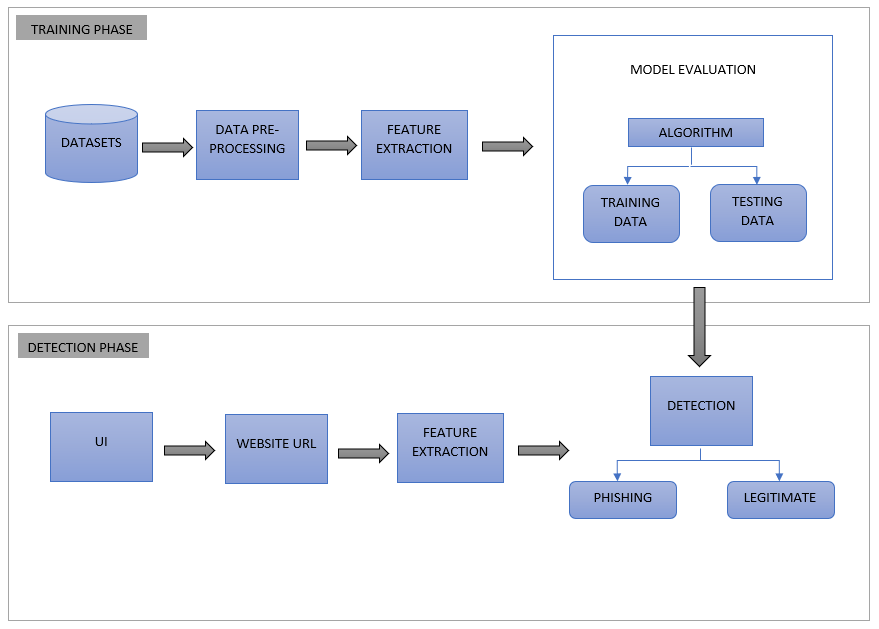
\includegraphics[scale=0.6]{newModel.png}}
\caption{System Architecture}
\label{fig}
\end{figure}
\par  In this section, we describe the phishing detection
framework which consists of two major parts as shown in Fig:3.1. The first part is the Training Phase and the second part is the Detection Phase. In
the first phase, datasets containing urls are prepared for the machine learning algorithm and model is evaluated. In the second phase, an input url is received from the user and based on the evaluated model, the url is classified into phishing or legitimate.
\section{Training Phase}
\subsection{Dataset}
\par  A dataset is a collection of structured or unstructured data that is organized and labeled for specific tasks. Datasets serve as the foundation for training and evaluating machine learning models, conducting statistical analysis, and extracting meaningful insights from data.
\par The dataset is created by merging two different datasets to improve the efficiency of prediction.
\begin{enumerate}
    \item Dataset-I
\par This dataset is collected from phishtank.com which contains 96,020 data with 50\% phishing and 50\% of legitimate urls. This dataset contains columns - domain and label,where domain represents the urls and label denotes whether the url is phishing or legitimate by representing 1 and 0 respectively.
    
    \item Dataset-II
\par This dataset is collected from Kaggle.com which contains 450,176 data, having url, label and result as columns.
\end{enumerate}
\begin{figure}[H]
\centerline{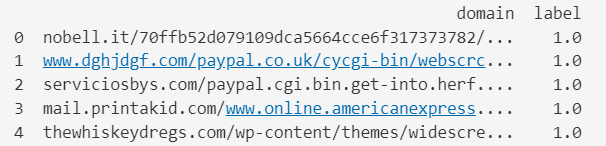
\includegraphics[scale=0.8]{dataset1.png}}
\caption{Dataset-I from phishtank.com}
\label{fig}
\end{figure}
\begin{figure}[H]
\centerline{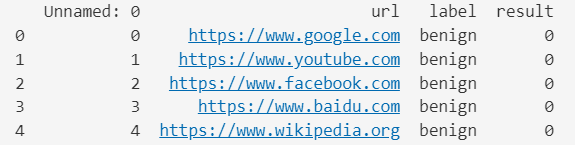
\includegraphics[scale=0.8]{dataset2.png}}
\caption{Dataset-II from kaggle.com}
\label{fig}
\end{figure}

\subsection{Data Pre-Processing}
\par
Data preprocessing is a crucial step in machine learning that involves transforming raw data into a suitable format for training machine learning models. It helps to improve the quality and reliability of the data, reduces noise and inconsistencies, and enhances the performance of the models.Here are some data preprocessing techniques used in our project :
\begin{enumerate}
  \item Data Cleaning: This step involves handling missing values, outliers, and duplicates in the data. Missing values can be imputed using techniques like mean, median, or mode. Outliers can be detected and treated using statistical methods or replaced with more reasonable values. Duplicates can be removed to avoid bias in the analysis.
  \item Data Reduction: Data reduction in preprocessing refers to the process of reducing the size or complexity of a dataset without losing critical information. It is often performed as an initial step in data preprocessing to address challenges such as computational limitations, storage constraints, or noise in the data. Data reduction techniques aim to retain the most relevant information while reducing redundancy and removing irrelevant or noisy data points. 
  \item Data Integration: Data integration in preprocessing refers to the process of combining multiple heterogeneous data sources into a unified and consistent format. It involves merging, transforming, and resolving inconsistencies in the data from different sources to create a comprehensive dataset for further analysis or modeling. Data integration is a critical step in data preprocessing when working with data from various systems, databases, or file formats. 
  
\end{enumerate}
\subsection{Feature Extraction}
\par Feature extraction in machine learning refers to the process of transforming raw input data into a set of meaningful and representative features that can be used as inputs for machine learning algorithms. The goal of feature extraction is to capture relevant information from the data and create a compact and informative representation that facilitates the learning process and improves the performance of the models.
\par Statistical measures can be computed from the raw data to capture important characteristics. These measures can include mean, median, standard deviation, variance, skewness, kurtosis, and other moments. Statistical measures provide insights into the distribution, central tendency, and spread of the data. Exploratory data analysis, domain expertise, and experimentation are often necessary to determine the most effective feature extraction methods for a given problem.
\par In this project, the features are classified into 2 categories:
\begin{itemize}
    \item Lexical Features
    \item Numerical Features
\end{itemize}

\subsection{Algorithm}

\subsubsection{Logistic Regression}
\par Logistic regression is a statistical modeling technique used for binary classification problems, where the goal is to predict the probability of an event or the likelihood of an outcome falling into one of two classes. Despite its name, logistic regression is a classification algorithm rather than a regression algorithm. It is based on the assumption that the relationship between the input variables (also known as independent or predictor variables) and the log-odds of the binary outcome (dependent or response variable) can be approximated by a linear relationship.
\par The logistic function, also called the sigmoid function, is used to map the linear combination of input variables to a range between 0 and 1, representing the probability of belonging to the positive class. The logistic function is given by:

p(x) = 1 / (1 + e\^(-z))

where p(x) is the predicted probability, x is the input variables, and z is the linear combination of the input variables.
\begin{figure}[H]
\centerline{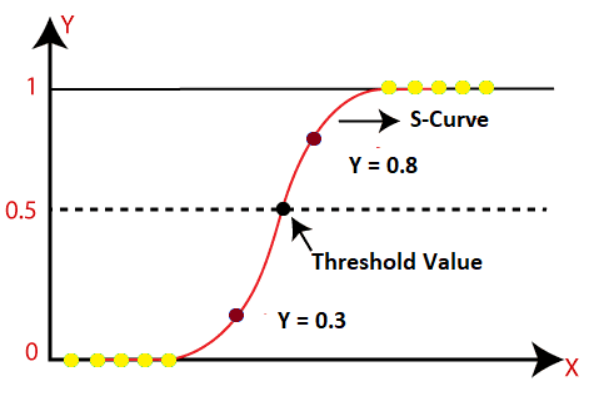
\includegraphics[scale=0.8]{LRgraph.png}}
\caption{Logistic Regression}
\label{fig}
\end{figure}
\section{Detection Phase}
\subsection{User Interface}
\par A user interface (UI) refers to the visual and interactive elements through which users interact with a software application or system. It provides a means for users to input commands or data and receive feedback or output from the system. The primary goal of a user interface is to create a user-friendly and intuitive experience, allowing users to efficiently and effectively interact with the software.
\subsubsection{Reactjs}
\par ReactJS, also known as React, is a popular JavaScript library for building user interfaces. It was developed by Facebook and is widely used for creating interactive and dynamic web applications. React follows a component-based architecture, where the UI is broken down into reusable and modular components, making it easier to develop and maintain complex user interfaces.
\subsubsection{Nodejs}
\par Node.js is an open-source JavaScript runtime environment built on Chrome's V8 JavaScript engine. It allows developers to run JavaScript code outside the browser, on the server-side, and build scalable and high-performance web applications. Node.js provides an event-driven, non-blocking I/O model that makes it lightweight and efficient, suitable for real-time applications and server-side programming.
\par Node.js can be used to build APIs (Application Programming Interfaces) for server-side development. APIs are used to define the endpoints and functionality of web services, allowing client applications to interact with the server and exchange data.

\subsection{Website URL}
\par A URL (Uniform Resource Locator) is a specific address that identifies a resource on the internet. It typically consists of several components, including the protocol, domain name, path, and possibly query parameters.
\begin{figure}[H]
\centerline{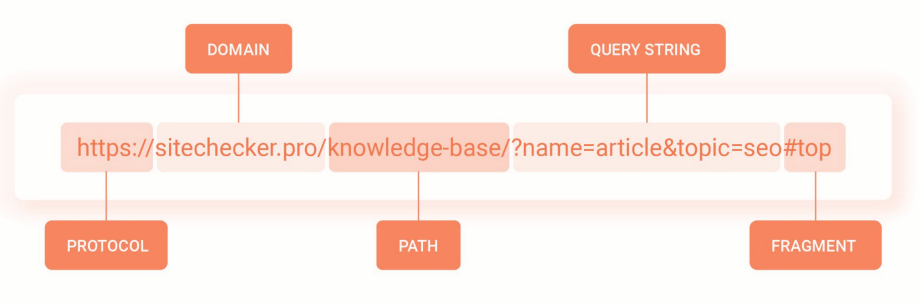
\includegraphics[scale=0.6]{features.png}}
\caption{Basic structure of a URL}
\label{fig}
\end{figure}

\subsection{Detection}
\par The input URL from the user interface is predicted either as Phishing or Non-Phishing.
\begin{itemize}
    \item Phishing: Type of URLs that are specifically designed to deceive users by impersonating legitimate websites or services.
    \item Non-Phishing Type of URLs that are the genuine URLs of legitimate websites or services.
\end{itemize}

\section{Objectives}

\begin{itemize}
    \item To extract features that can produce effective accuracy in model evaluation
\item To analyse the accuracy level for different machine learning algorithms and implementing the best among them
\item To design and Implement a Web Application to search and detect whether it is phishing or not.
\item To store URLs, which are detected as either phishing or non-phishing

\end{itemize}
\section{Scope}
\begin{itemize}
    \item Algorithm will analyze various blacklisted and legitimate URL features to accurately detect the phishing websites including zero-hour phishing websites.

\end{itemize}

\section{System Requirements}
\subsection{  Software Requirements  }
\renewcommand{\labelitemi}{}

\begin{itemize}
    \item \textbf{Programming Languages:} Python, JavaScript
    \item \textbf{Integrated Development Environment (IDE):}VisualStudioCode, Google Colab
    \item \textbf{Libraries:} numpy, panda, scikit-learn, Matplotlib/Seaborn, pycaret, pickle, React
    \item \textbf{Frameworks:} Anaconda, Express.js
    \item \textbf{Web Browsers:} Google Chrome, Mozilla Firefox,Microsoft Edge
    \item \textbf{Package Managers:} pip, npm
    \item \textbf{Version Control:} Git, Github
\end{itemize}


\subsection{Hardware Requirements}
\begin{itemize}
    \item \textbf{Processor:} Intel i5 and above
    \item \textbf{RAM:} 8gb and above
\end{itemize}






















%
\chapter{SYSTEM IMPLEMENTATION }
\thispagestyle{empty}
\\

\par The implementation is divided into five parts.
\begin{enumerate}
    \item Data Pre-processing
    \item Feature Extraction
    \item Model Comparison
    \item Model Evaluation
    \item Model Implementation
\end{enumerate}

\section{DATA PRE-PROCESSING}
\par Data pre-processing is an essential step in preparing raw data for analysis and machine learning tasks. It involves transforming and cleaning the data to ensure its quality, consistency, and suitability for further analysis.
We obtained two separate datasets from different sources and merged them to create a larger dataset for training and testing our machine learning models.
\subsubsection{Data Cleaning}
\par In the Dataset-I (url and label as columns), we found 92 urls without any corresponding label values i.e, having null values. and these rows were dropped from this datasets.
\subsubsection{Data Reduction}
We only need the urls and there corresponding label values(1 0r 2 representing phishing or legitimate) as the input datas, the Dataset-II contains unwanted columns so they are also dropped.
\subsubsection{Data Integration}
Next we will be merging our 2 datasets , for that we will be considering the Datatypes and names of the columns to avoid damage of the resultant dataset after merging. Merging DataFrames with different data types for the same column name might lead to inconsistencies and unexpected behavior and merging DataFrames having different column names produce splitting of the values. So they both are handled before merging. After Merging we obtained a dataset having 546,104 datas and saved in a new csv file.

\par After merging there are chances of having duplicate data inside the resultant dataset. There were 194 Duplicate URLs in our resultant dataset. And these were dropped. Fig 4.2 shows the 
Bar-Graph Classification of Phishing and Legitimate urls inside the new dataset:

\begin{figure}[H] 
  \centering
  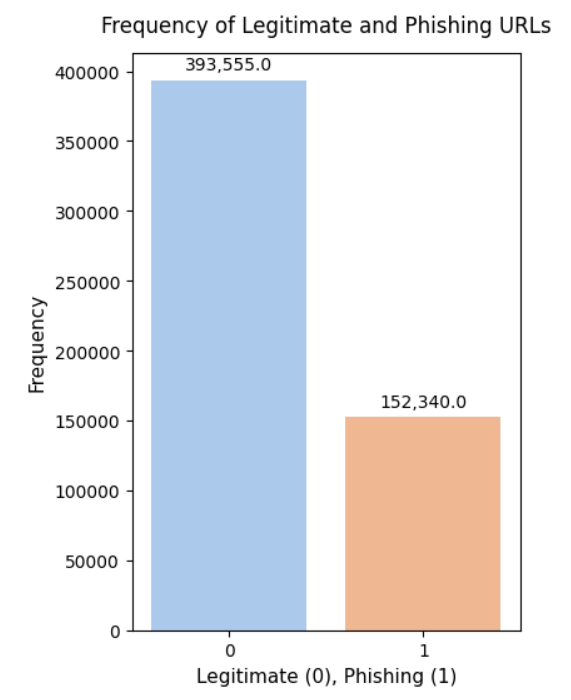
\includegraphics[scale=0.6]{barGraph_PorL.png} 
  \caption{Bar-Graph Classification of Phishing and Legitimate data.}
  \label{fig}
\end{figure}

\begin{figure}[H] 
  \centering
  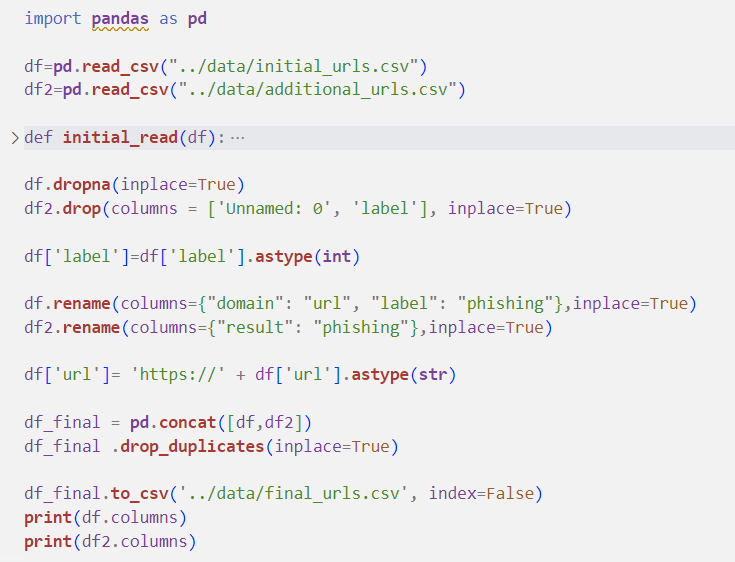
\includegraphics[scale=0.68]{DataPreprocessing_Code.png} 
  \caption{Data Pre-Processing}
  \label{fig}
\end{figure}

\section{FEATURE EXTRACTION}
\par Feature extraction is a technique used to reduce the dimensionality of data by transforming the raw input into a set of derived features that capture the essential information. It aims to highlight the most relevant aspects of the data and discard irrelevant or redundant information. 
\par In our project, the features are generally classified into two:
\begin{enumerate}
  \item Lexical Features
  \item Numerical Features
\end{enumerate}
\subsection{Lexical Features}
\par Lexical features in URL feature extraction involve analyzing the textual components and patterns within a URL. These features capture characteristics related to the structure, keywords, symbols, and other textual elements of a URL.
\begin{itemize}
  \item getEntropy :-{ It is known that DGA(Domain Generation Algorithm) domains have a greater level of disorderliness in their alphabetic distribution. Legitimate domains tend to have well-defined names that speak to a brand or a product so tend to be less disorganized. Thus, measuring the entropy of URL strings tells us which domain names are ‘not-so-real.}
  \item hasLogin :-{Check if the URL contains specific keyword "login," .We can capture the fact that certain ‘red flag’ keywords appear in a URL string. These keywords may relate to keywords attackers use when trying to spoof a legitimate page or keywords that relate to popular nomenclature of security settings on a website that a hacker will try to manipulate.So,If the URL string contains “login” keyword, the value assigned to this feature is 1 (phishing) or else 0 (legitimate).}
  \item Redirection :-{ Phishing attackers often employ redirection techniques to hide the true destination of a malicious URL. By redirecting users through multiple URLs or using URL shorteners, they can make it more difficult for users and security systems to identify the final destination. Checks the presence of "//" in the URL. The existence of “//” within the URL path means that the user will be redirected to another website.(avoiding the "//" after the http/https)=}
  \item lenClassify :-{Computes the length of the URL. Phishers can use long URL to hide the doubtful part in the address bar. In this project, if the length of the URL is greater than or equal 54 characters then the URL classified as phishing otherwise legitimate. If the length of URL >= 54 , the value assigned to this feature is 1 (phishing) or else 0 (legitimate).}
  \item haveAtSign :-{Checks for the presence of '@' symbol in the URL. Using “@” symbol in the URL leads the browser to ignore everything preceding the “@” symbol and the real address often follows the “@” symbol.And also used to mimic or spoof well-known websites or services. If the URL has '@' symbol, the value assigned to this feature is 1 (phishing) or else 0 (legitimate).}
  \item getDepth :-{The depth of a URL refers to the number of hierarchical levels or directories in the URL's path. It represents how nested a specific resource is within a website's directory structure. This feature calculates the number of sub pages in the given url based on the '/'.}
  \item tinyURL :-{URL shortening is a method in which a URL are shortened and can still lead to the required webpage. And this is accomplished by most of the phishing websites.If the URL is using Shortening Services, the value assigned to this feature is 1 (phishing) or else 0 (legitimate).}
  \item isDomainIp :-{Some Phishing URLs represents the domain name by IP address instead of hostname. Checks for the presence of IP address in the URL. URLs may have IP address instead of domain name. If an IP address is used as an alternative of the domain name in the URL, we can be sure that someone is trying to steal personal information with this URL.If the domain part of URL has IP address, the value assigned to this feature is 1 (phishing) or else 0 (legitimate).}
  \item prefixSuffix :-{Checking the presence of '-' in the domain part of URL. The dash symbol is rarely used in legitimate URLs. Phishers tend to add prefixes or suffixes separated by (-) to the domain name so that users feel that they are dealing with a legitimate webpage.If the URL has '-' symbol in the domain part of the URL, the value assigned to this feature is 1 (phishing) or else 0 (legitimate).}
\end{itemize}

\begin{figure}[H]
  \centering
  {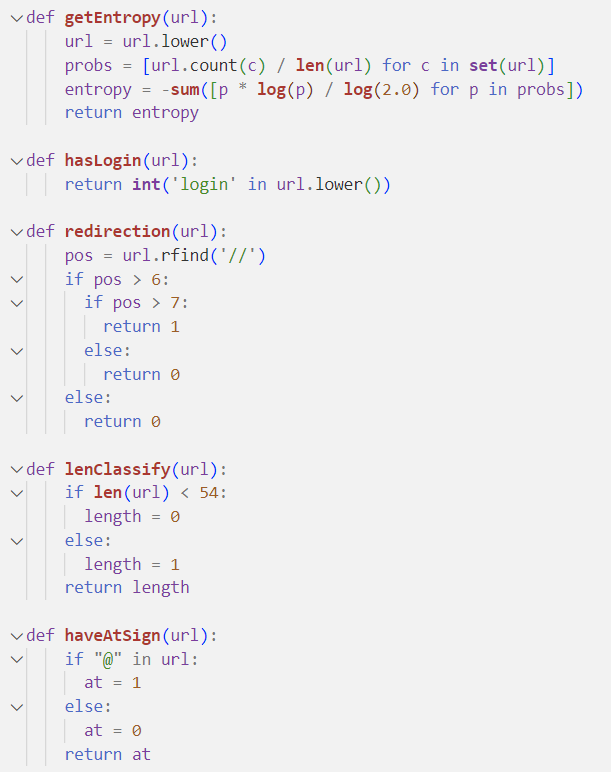
\includegraphics[width=0.45\textwidth]{featureExtraction_Code1.1.png}\label{fig:figure1}}
  \hfill
  {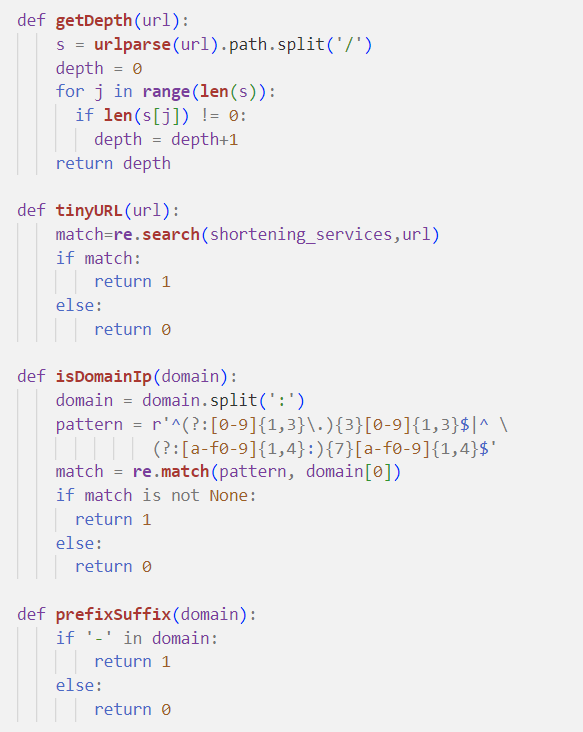
\includegraphics[width=0.450\textwidth]{featureExtraction_Code1.2.png}\label{fig:figure2}}
  \caption{Lexical Feature Extraction}
  \label{fig:bothfigures}
\end{figure}

\subsection{Numerical Features}
\par Numerical value-based features are features that represent quantitative or continuous values. These features can take on a wide range of numeric values and are often used in various machine learning algorithms and statistical analyses. 


\par Features of a URL are basically classified into - protocol, domain, path, query, fragment. The length of this each features and the count of the different special characters in that specific feature are extracted. The special characters like  ‘.’ ‘-’ ‘/’ ‘?’ ‘=’ ‘@’ ‘\&’ ‘!’ ‘\ ’ ‘{~}' ‘,’ ‘+’ ‘*’ ‘\#’ ‘\$’ ‘\%’ .
\par These features are :\\ 
{\footnotesize 
\begin{multicols}{3} % Set the number of columns you want
\begin{itemize}
\item url\_length
\item qty\_dot\_url
\item qty\_hyphen\_url
\item qty\_slash\_url
\item qty\_questionmark\_url
\item qty\_equal\_url
\item qty\_at\_url
\item qty\_and\_url
\item qty\_exclamation\_url
\item qty\_space\_url
\item qty\_tilde\_url
\item qty\_comma\_url
\item qty\_plus\_url
\item qty\_asterisk\_url
\item qty\_hashtag\_url
\item qty\_dollar\_url
\item qty\_percent\_url
\item domain\_length
\item qty\_dot\_domain
\item qty\_hyphen\_domain
\item path\_length
\item qty\_dot\_path
\item qty\_hyphen\_path
\item qty\_slash\_path
\item qty\_equal\_path
\item qty\_at\_path
\item qty\_and\_path
\item qty\_exclamation\_path
\item qty\_space\_path
\item qty\_tilde\_path
\item qty\_comma\_path
\item qty\_plus\_path
\item qty\_asterisk\_path
\item qty\_dollar\_path
\item qty\_percent\_path
\item query\_length
\item qty\_dot\_query
\item qty\_hyphen\_query
\item qty\_slash\_query
\item qty\_questionmark\_query
\item qty\_equal\_query
\item qty\_at\_query
\item qty\_and\_query
\item qty\_exclamation\_query
\item qty\_space\_query
\item qty\_tilde\_query
\item qty\_comma\_query
\item qty\_plus\_query
\item qty\_asterisk\_query
\item qty\_dollar\_query
\item qty\_percent\_query
\item fragment\_length
\item qty\_dot\_fragment
\item qty\_hyphen\_fragment
\item qty\_slash\_fragment
\item qty\_questionmark\_fragment
\item qty\_equal\_fragment
\item qty\_and\_fragment
\item qty\_exclamation\_fragment
\item qty\_space\_fragment
\item qty\_comma\_fragment
\item qty\_asterisk\_fragment
\item qty\_hashtag\_fragment
\item qty\_dollar\_fragment
\item qty\_percent\_fragment
\end{itemize}.
\end{multicols}
}
\par Finally, a total of 74 features are extracted in this project. After extracting both the Lexical and Numerical Features, they are saved to a new csv file for the Model Evaluation.
\begin{figure}[H]
\centerline{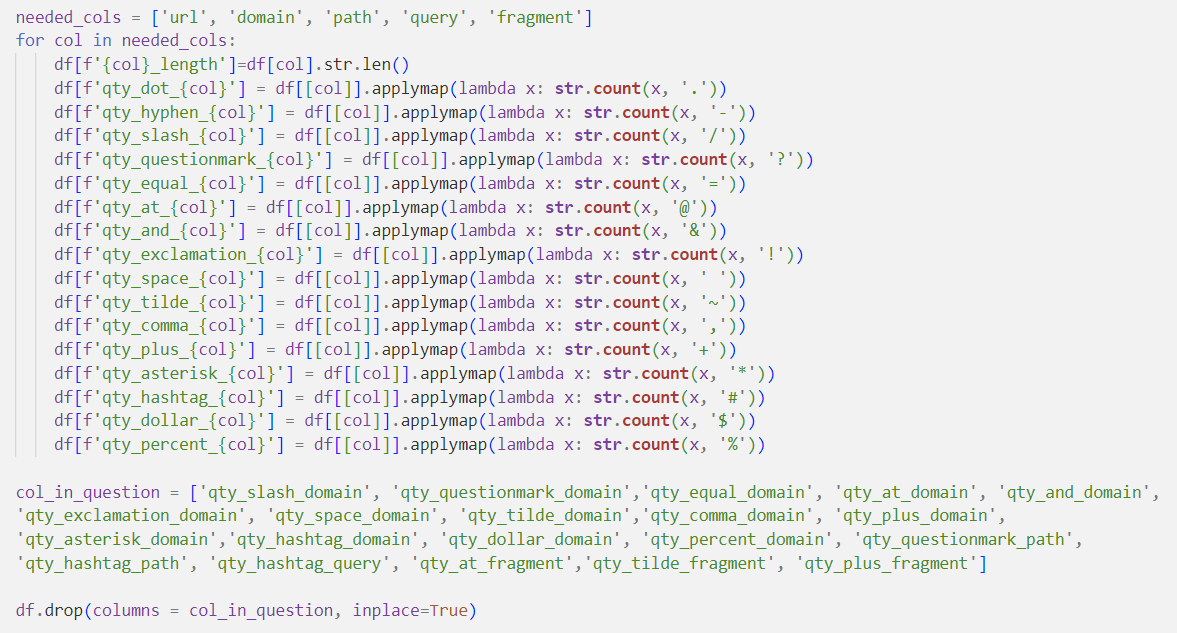
\includegraphics[scale=0.55]{featureExtraction_Code2.png}}
\caption{Numerical Feature Extraction}
\label{fig}
\end{figure}


\section{MODEL COMPARISON}
\subsection{Pycaret}
\par PyCaret is a Python library that provides an easy-to-use interface for training and comparing multiple machine learning models. It offers a variety of functions and tools to streamline the model development process and make it efficient. We use this library to compare the different machine learning models by using the extracted features and it will returns a table of model performance metrics sorted by  specified evaluation metrics - accuracy, AUC, recall, precision, F1, Kappa and MCC.

\par 15 different algorithms were compared and Logistic Regression(94.45\%) gave more accuracy among them. Thus, Logistic Regression model is used for testing and training the features. 
\begin{figure}[H]
\centerline{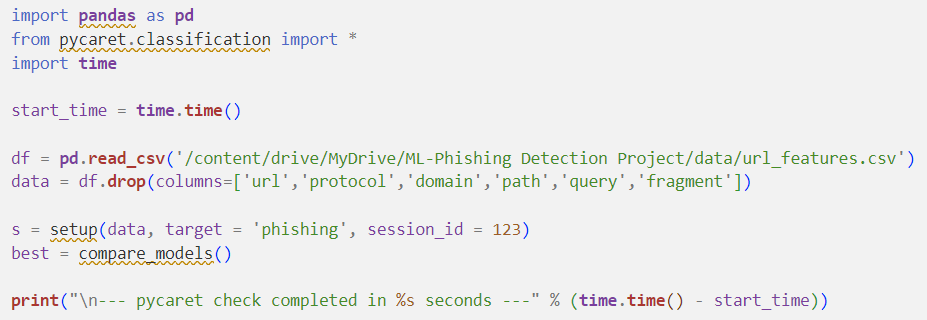
\includegraphics[scale=0.6]{pycaretCode.png}}
\caption{Pycaret Comparison}
\label{fig}
\end{figure}



\section{MODEL EVALUATION}
\par Model evaluation is a crucial step in machine learning to assess the performance and effectiveness of a trained model. It involves quantitatively measuring how well the model generalizes to new, unseen data and how accurately it predicts the target variable.Based on the model comparison, we evaluated the logistic regression(lr) model in this project.
\\
\par Evaluating a LR model includes the following steps:
\begin{itemize}
\item Spliting the dataset: Dividing dataset into training and testing sets, ensuring that both sets have a representative distribution of the target variable.
\item Training the LR model: Fiting the logistic regression model to the training data using a suitable library such as scikit-learn.
\item Make predictions: Use the trained model to predict the target variable for the test dataset.
\item Calculating evaluation metrics: Comparing the predicted values with the actual values from the test dataset and calculating the evaluation metrics such as accuracy, precision, recall, F1-score, AUC-ROC, and confusion matrix. Libraries like scikit-learn provide functions to calculate these metrics.
\end{itemize}

\begin{figure}[H]
\centerline{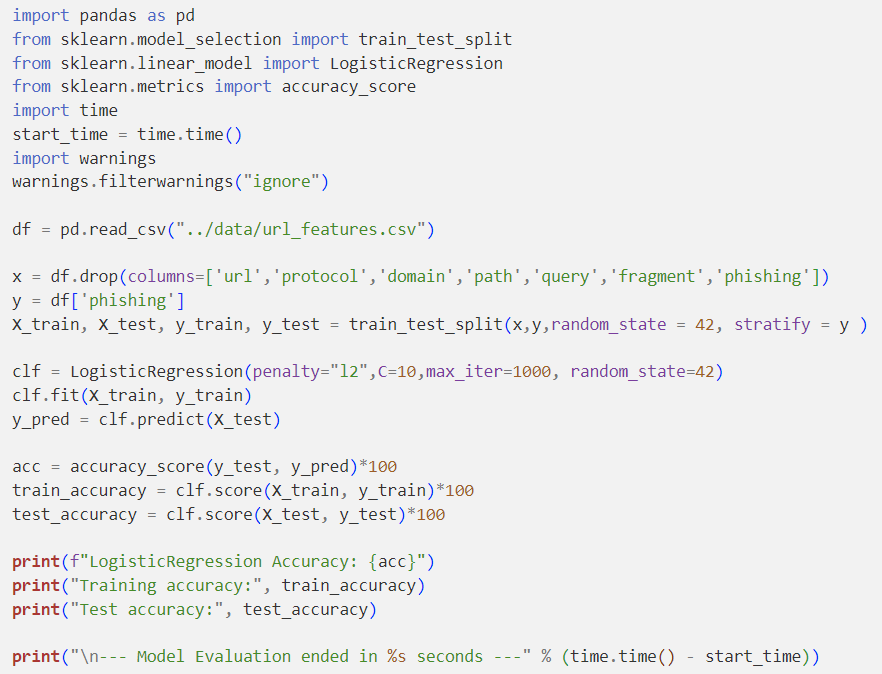
\includegraphics[scale=0.6]{modelEvaluation_Code.png}}
\caption{Model Evaluation}
\label{fig}
\end{figure}

\section{MODEL IMPLEMENTATION}
\par This phase involves deploying and integrating the trained machine learning model into a production environment where it can be used to make predictions on new, unseen data.This includes the following processes:
\begin{itemize}
\item Exporting the Model: Saving the trained model in a serialized format that can be easily loaded and used for predictions. We will be using python pickle module for exporting the trained lr model, which is a built-in module that provides a way to serialize and deserialize Python objects.
\item Model Integration: Integrating the model into the target application which is the WhalingGuard Web Appication where it will be used for predictions by API call.
\item Model Loading: Loading the serialized model into the implementation environment, making it ready for use. Again the pickle module is used to deserialize the model.
\item Input Data Feeding: Providing the new data, which is the URL to the model for prediction. This is done by passing the input data through a API call from the WhalingGuard User-Interface.
\item Feature Extraction: Extract the 74 different features from the input URL that where extracted during training phase. And saving that features to a new file for predicting.
\item Prediction Generation: Utilize the loaded model to generate predictions on the extracted features. Fiting the loaded model to the extracted features.  
\item Output Delivery: The prediction result is then passed to the API and the API then sends the results as a response to the frontend. The prediction results is also saved in csv file in the server, continously for each API calls.Then, at the user interface, the users can view the results whether the entered url is phishing or non-phishing.
\end{itemize}

\begin{figure}[H]
  \centering
  \subfloat[api.js]{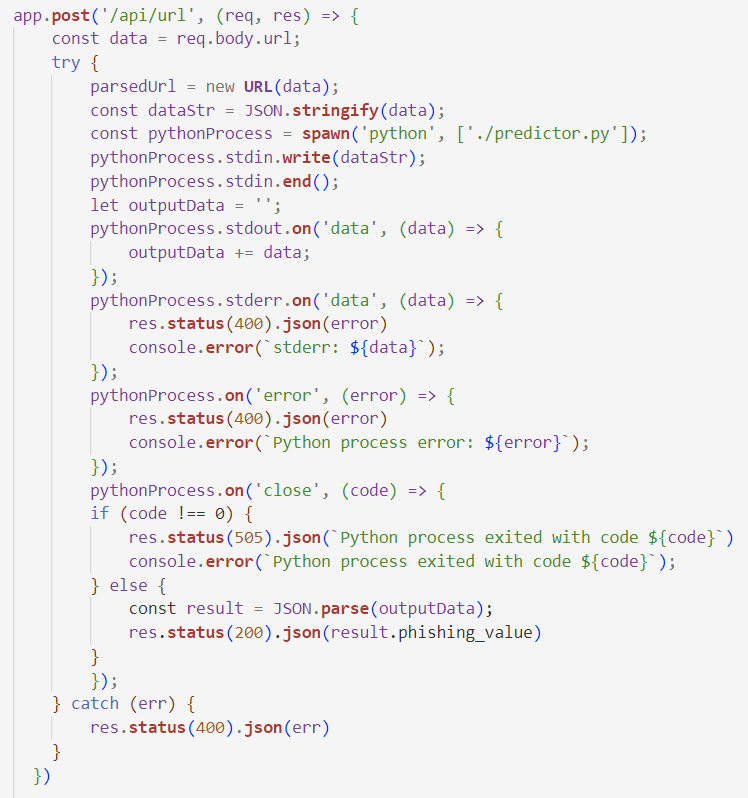
\includegraphics[width=0.47\textwidth]{apiCode.png}\label{fig:figure1}}
  \hfill
  \subfloat[predictor.py]{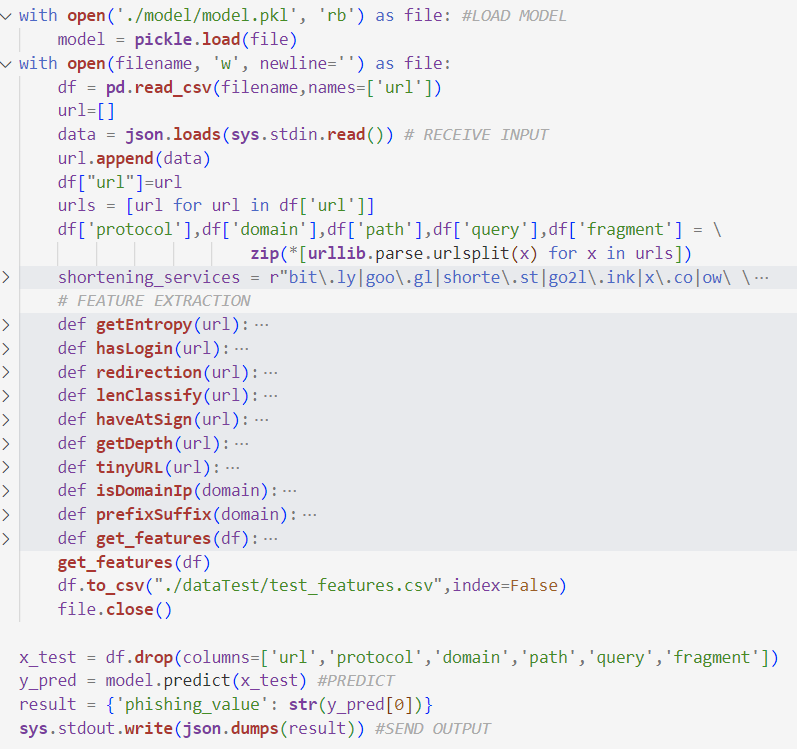
\includegraphics[width=0.47\textwidth]{predictorCode.png}\label{fig:figure2}}
  \label{fig:bothfigures}
\end{figure}

%\chapter{RESULTS AND DISCUSSIONS}
\thispagestyle{empty}
\onehalfspacing
\pagestyle{fancy}
\fancyhf{}
\fancyhead[LE,RO]{\textit{\footnotesize \thepage}}
\fancyhead[RE,LO]{\textit{\footnotesize Avenue - Online Event Management System}}
%\fancyfoot[LE,LO]{\textit{\footnotesize Department of CSE}}
\fancyfoot[LE,RO]{\textit{\footnotesize Department of CSE}}
 
\renewcommand{\headrulewidth}{2pt}
\renewcommand{\footrulewidth}{1pt}
\section{ Results   }
\subsection{Home Page}
This is the first interface for the Avenue event management system. This interface can be
accessed by all the system users and has information about what has to be done to access
the different system functionalities
\begin{figure}[h]
	\centering
	\includegraphics[scale=0.11]{HomePage1.png}
	\includegraphics[scale=0.11]{HomePage2.png}
	\caption{Home Page}
	\label{Home Page}
\end{figure}
\subsection{Client Login/Signup Page}
The client must login into his account for booking any events. If he does'nt have an account, he must create one by signing up.
\begin{figure}[H]
	\centering
	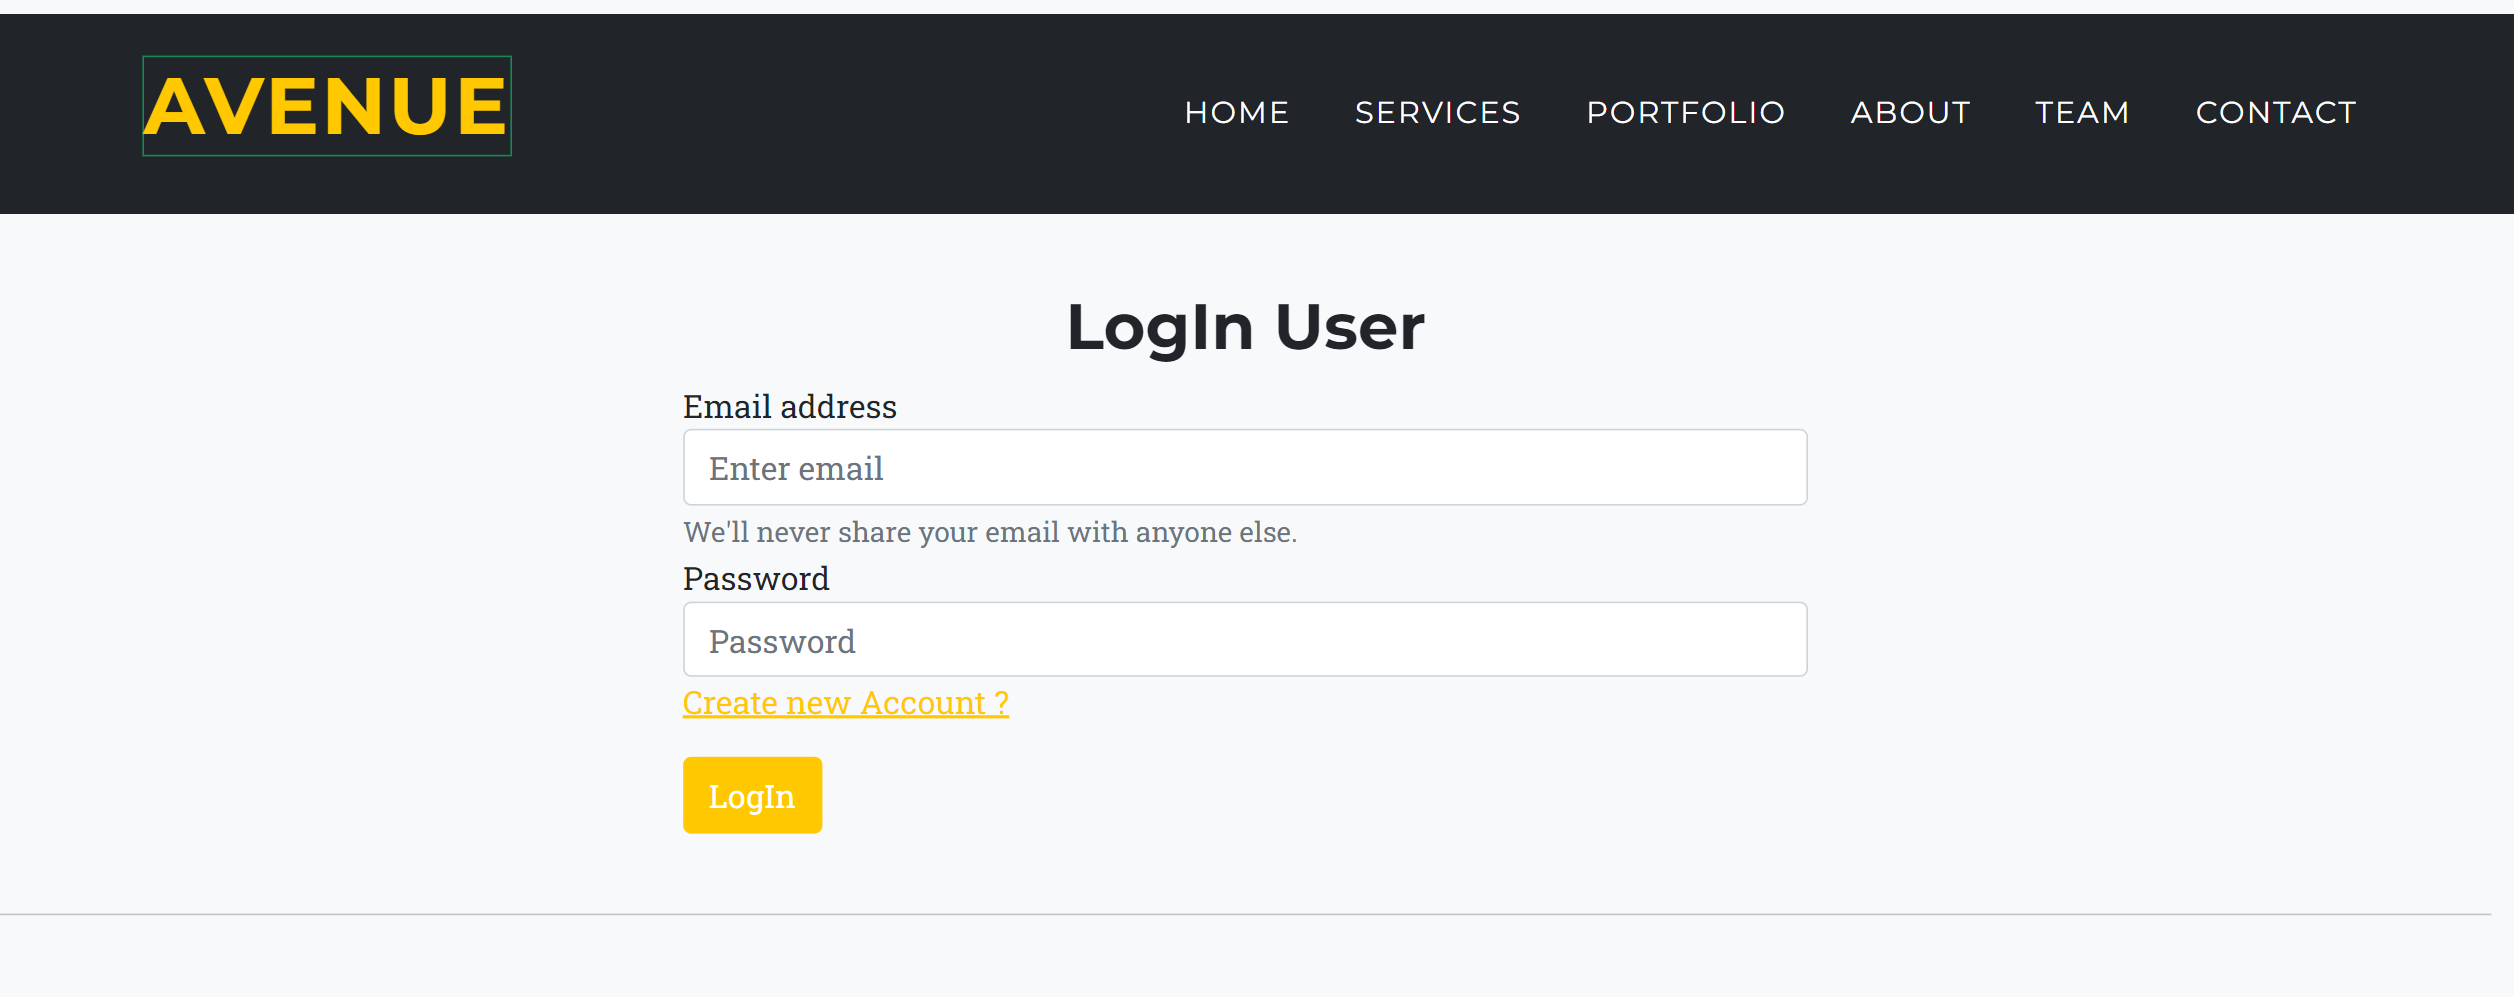
\includegraphics[scale=0.2]{login.png}\newline\newline
	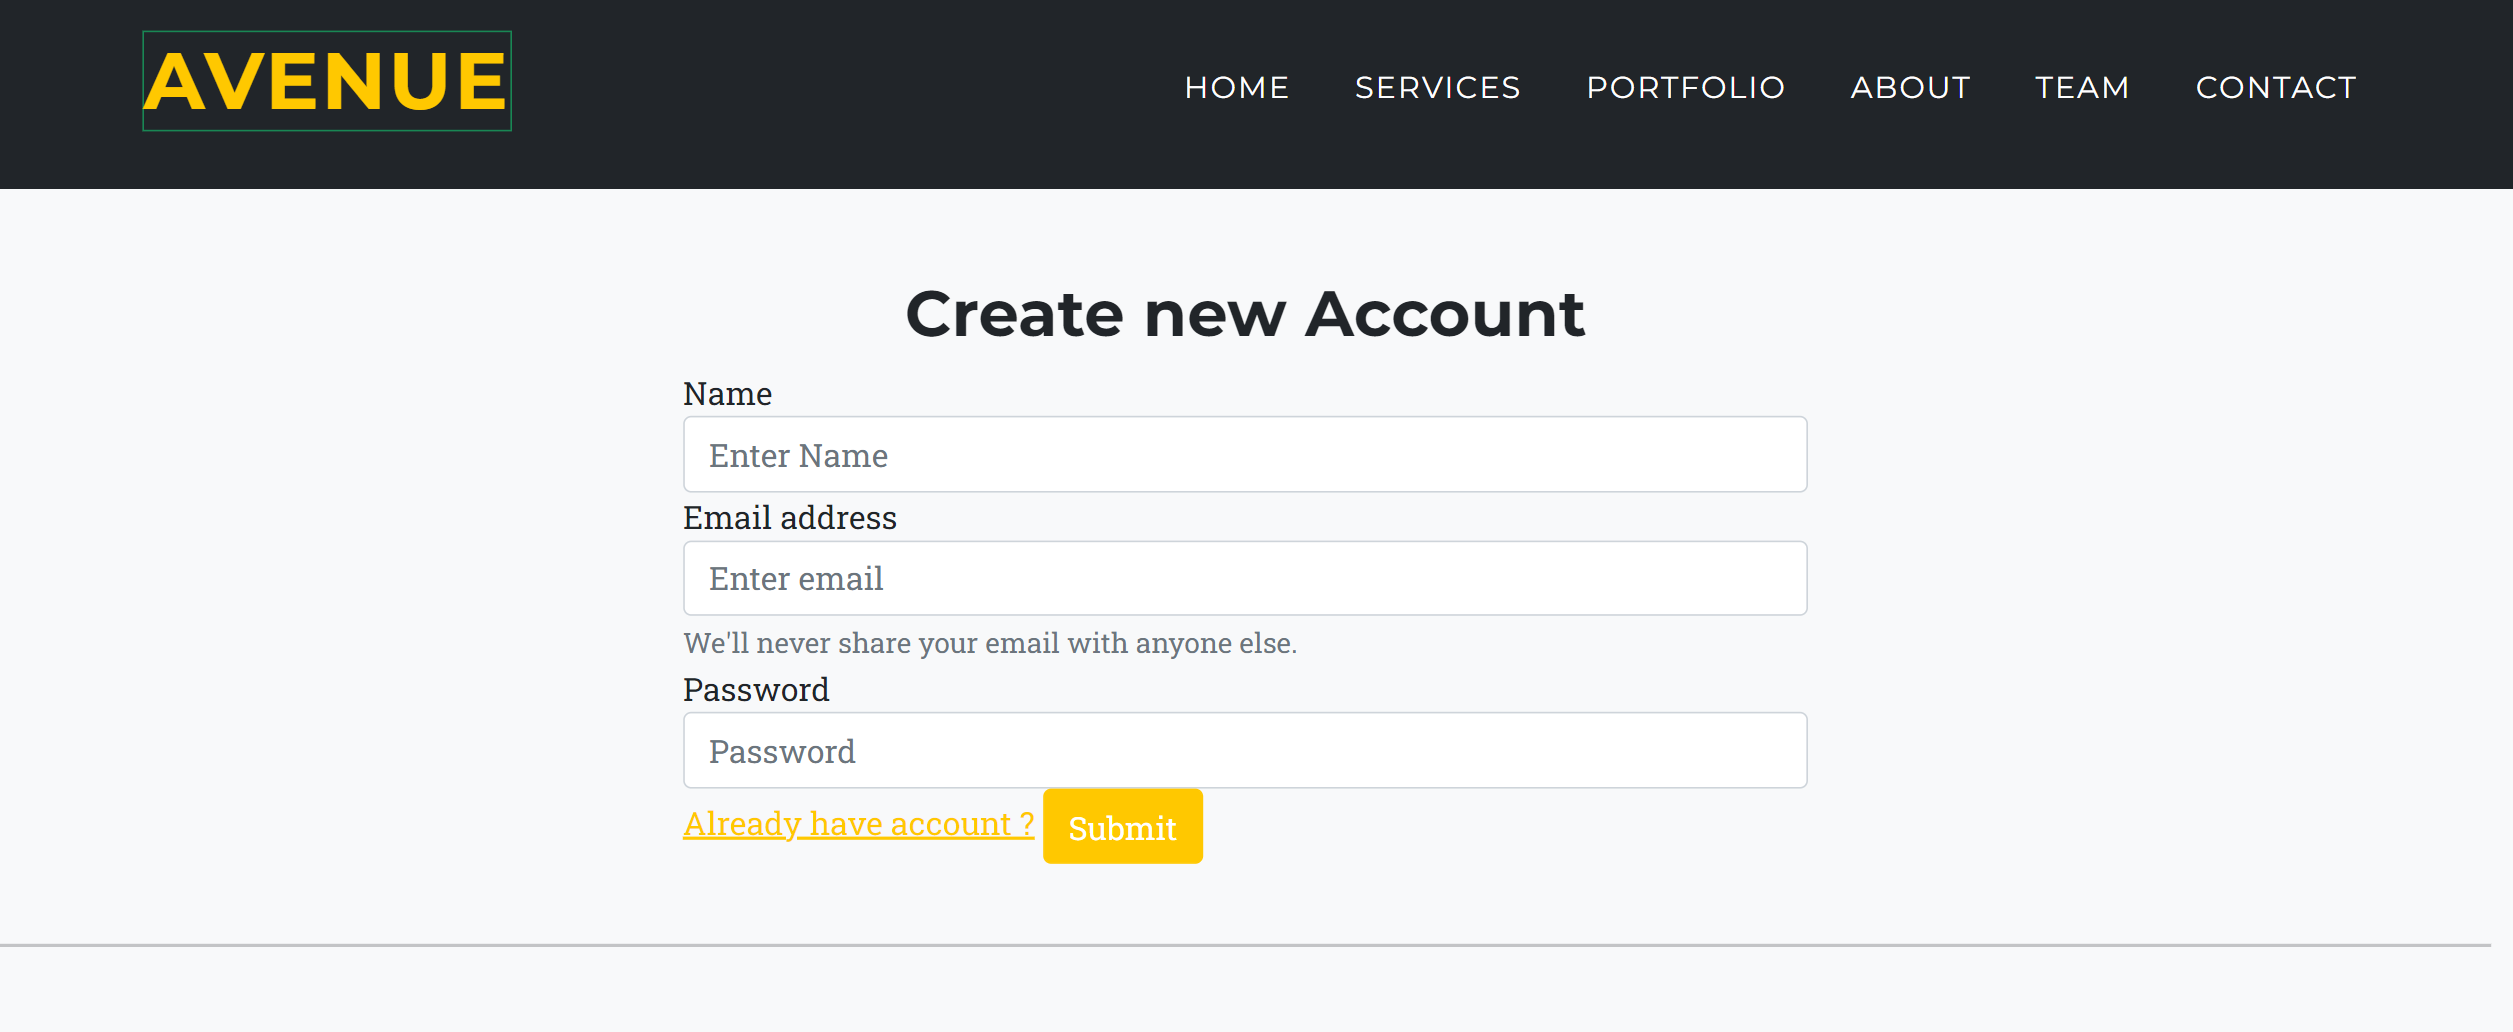
\includegraphics[scale=0.2]{signup.png}
	\caption{Login/Signup Page}
	\label{Login/Signup Page}
\end{figure}
\subsection{Client Booking Page}
The client will login after signing up and make a booking through this page as indicated
in the figure below. 
\begin{figure}[H]
	\centering
	\includegraphics[scale=0.17]{Contact.png}
	\caption{Booking Page}
	\label{Booking Page}
\end{figure}
\subsection{Event Planners Login and Account}
Event planners can login to their account where he can view his events and chat with his clients. He can also edit his profile details int the member account page.
\begin{figure}[H]
	\centering
	
\includegraphics[scale=0.33]{memberlogin.png}
\end{figure}
\begin{figure}[H]
	\centering
	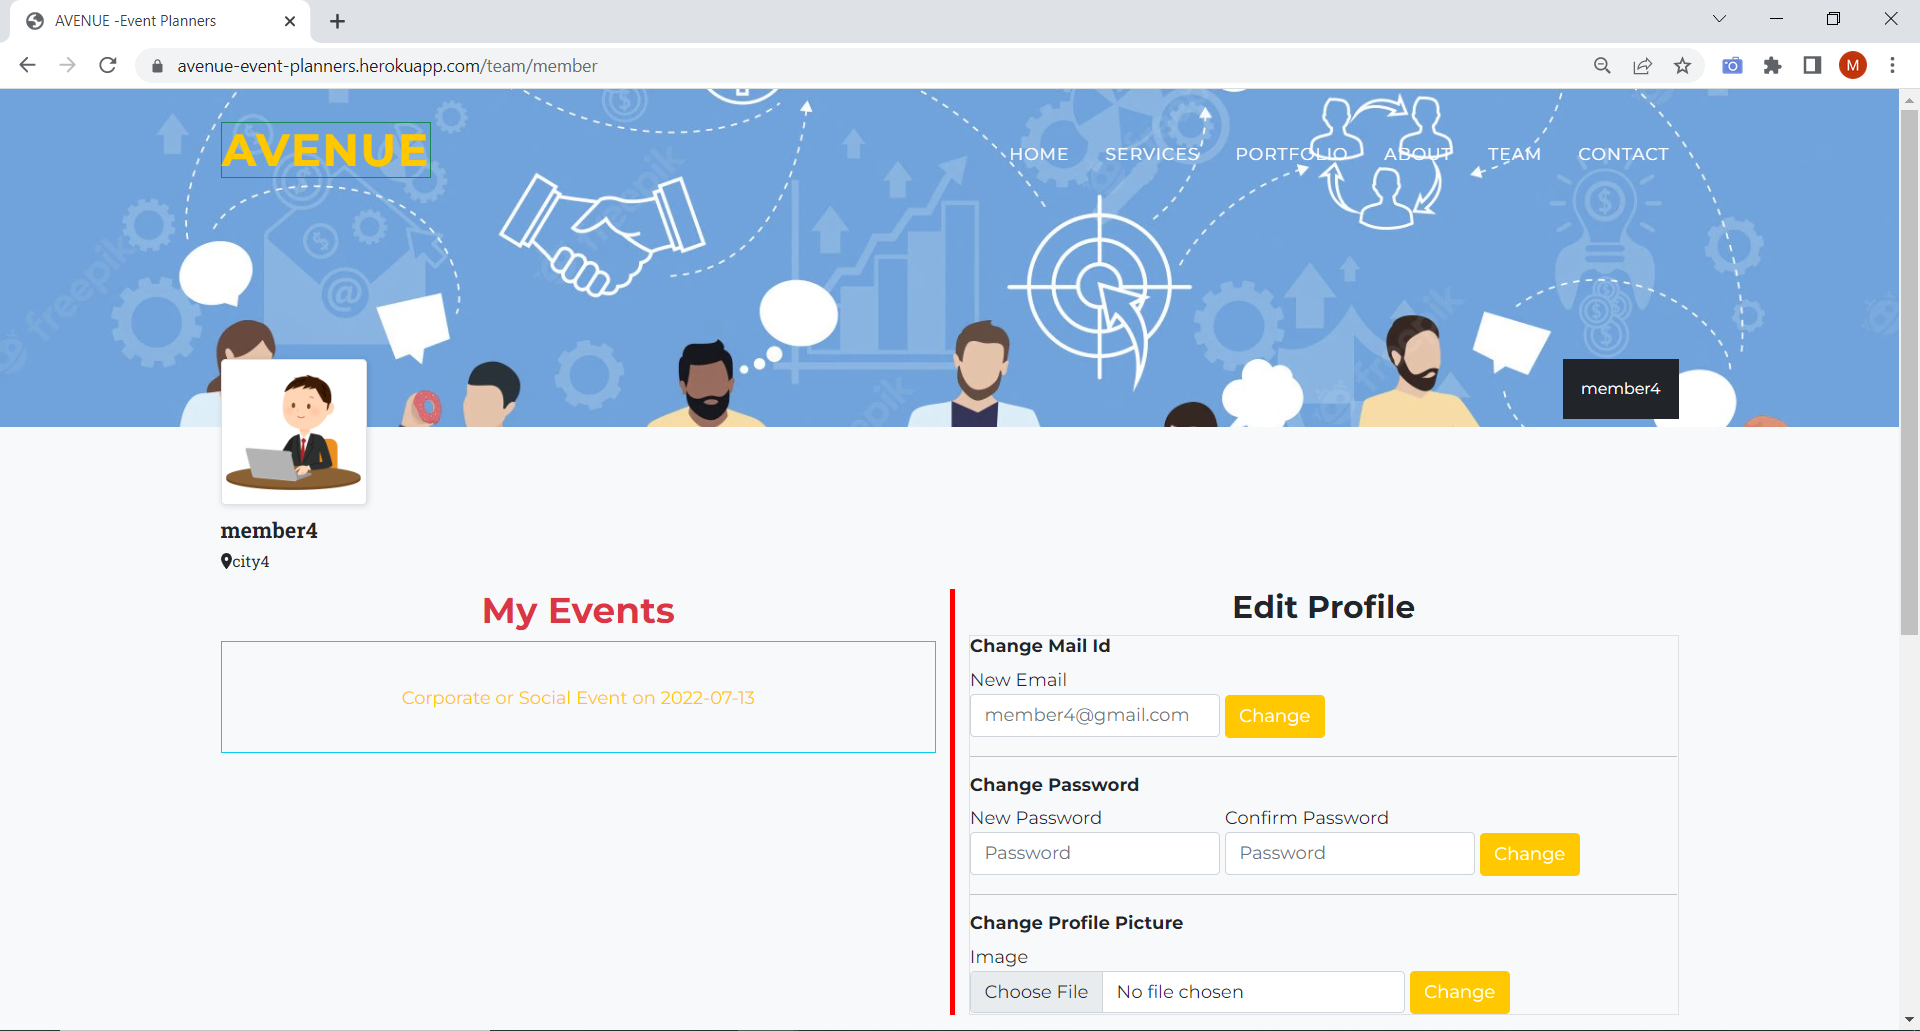
\includegraphics[scale=0.35]{memberaccount.png} \\
	\caption{Event Planners Login and Account Pages}
	\label{Event Planners Login and Account Pages}
\end{figure}
\subsection{Admin Login Interface}
Admin Login page is available in ' /admin ' route ,i.e, "BASE-URL/admin".Admin login details are matched with the login credentials already saved in the database.
\begin{figure}[H]
	\centering
	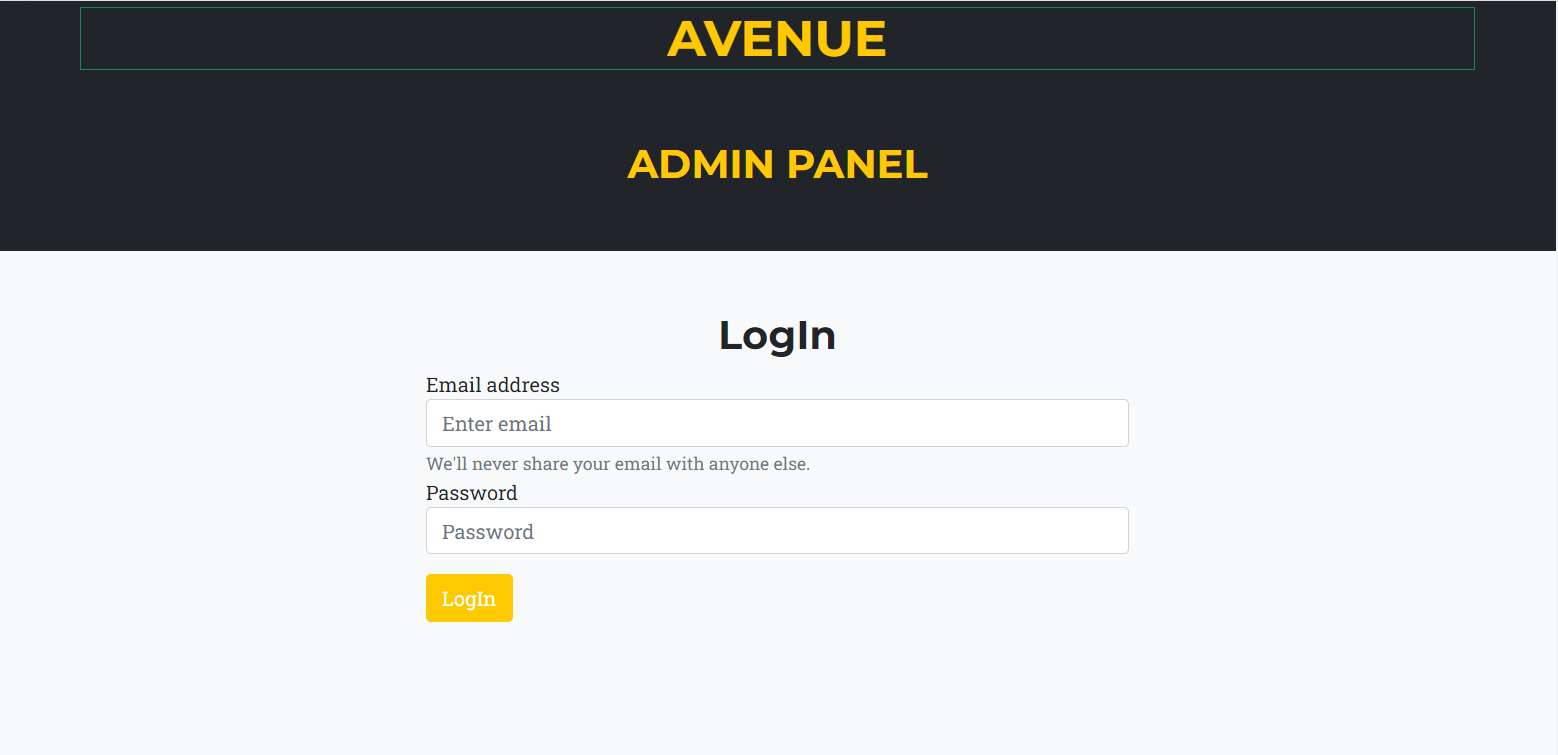
\includegraphics[scale=0.25]{adminlogin.png}
	\caption{Admin Login Page}
	\label{Admin Login Page}
\end{figure}
\subsection{Admin Panel Interface}
When the Username and Password is correct and the user privilege level is
Administrator, the user is then directed to the admin main switch board as indicated
below. 
\begin{figure}[H]
	\centering
	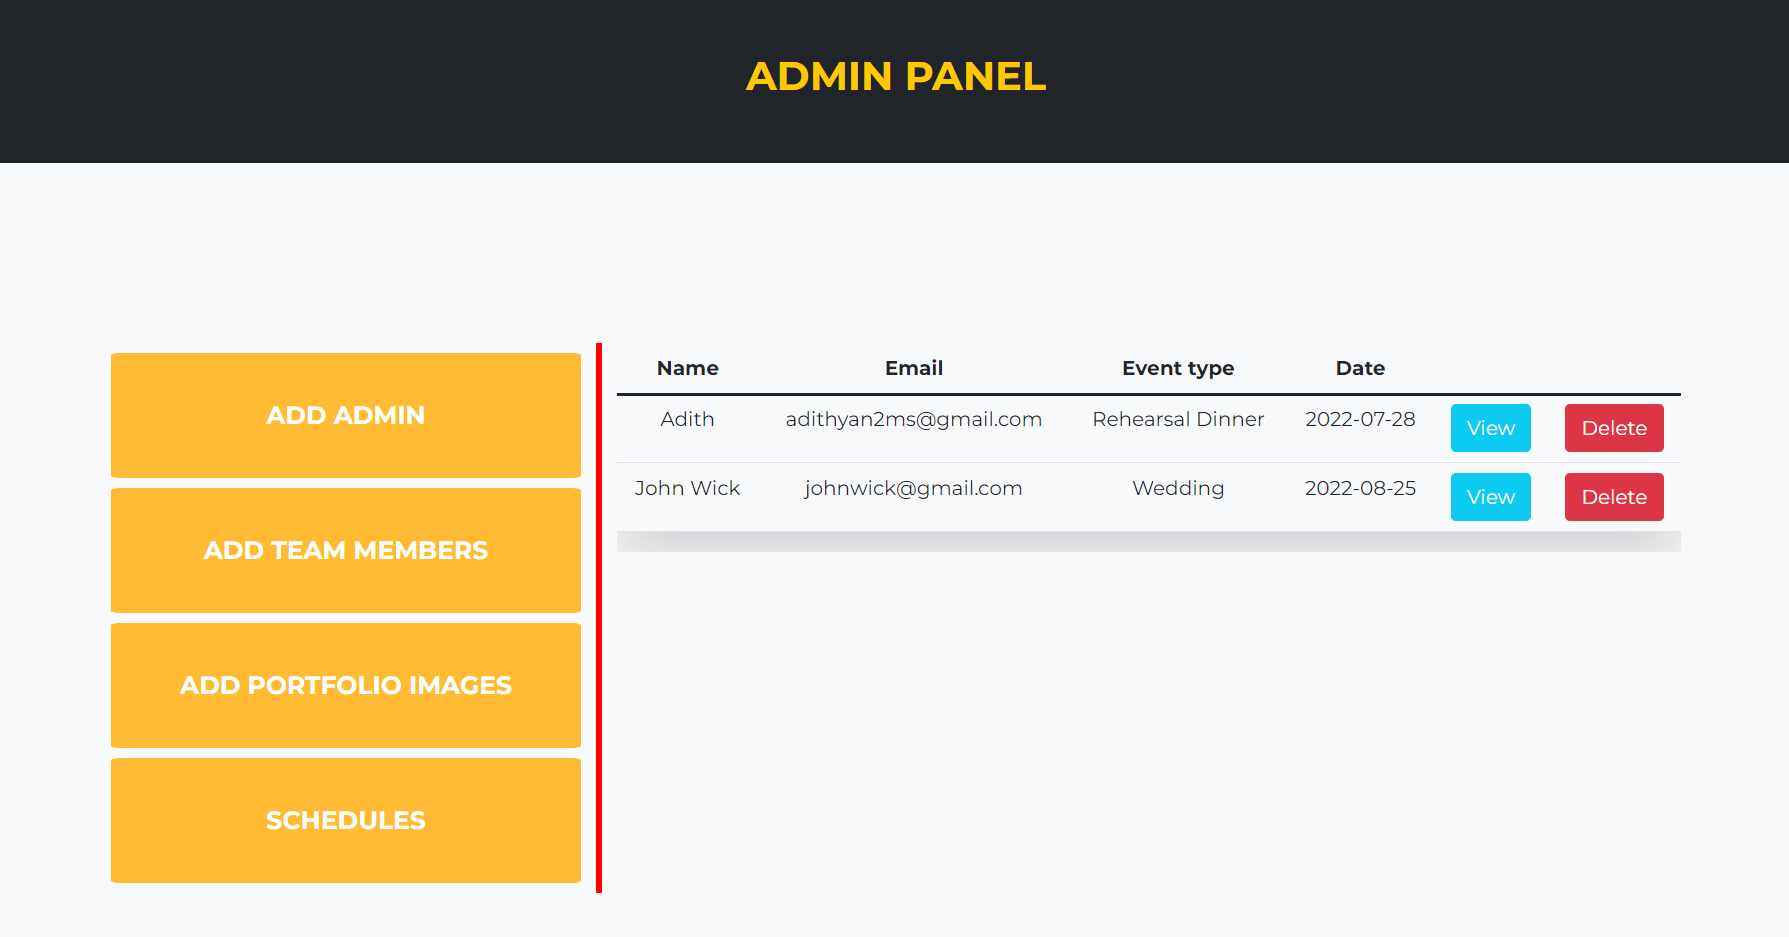
\includegraphics[scale=0.25]{adminhome.png}
	\caption{Admin Panel}
	\label{Admin Panel}
\end{figure}
\subsection{Admin Handling Requested Events}
Admin views all the event requests and accepts or rejects them based on certain circumtances like unavailability of members ,frank details etc.He also sets the event handling team before accepting the event.
\begin{figure}[H]
	\centering
	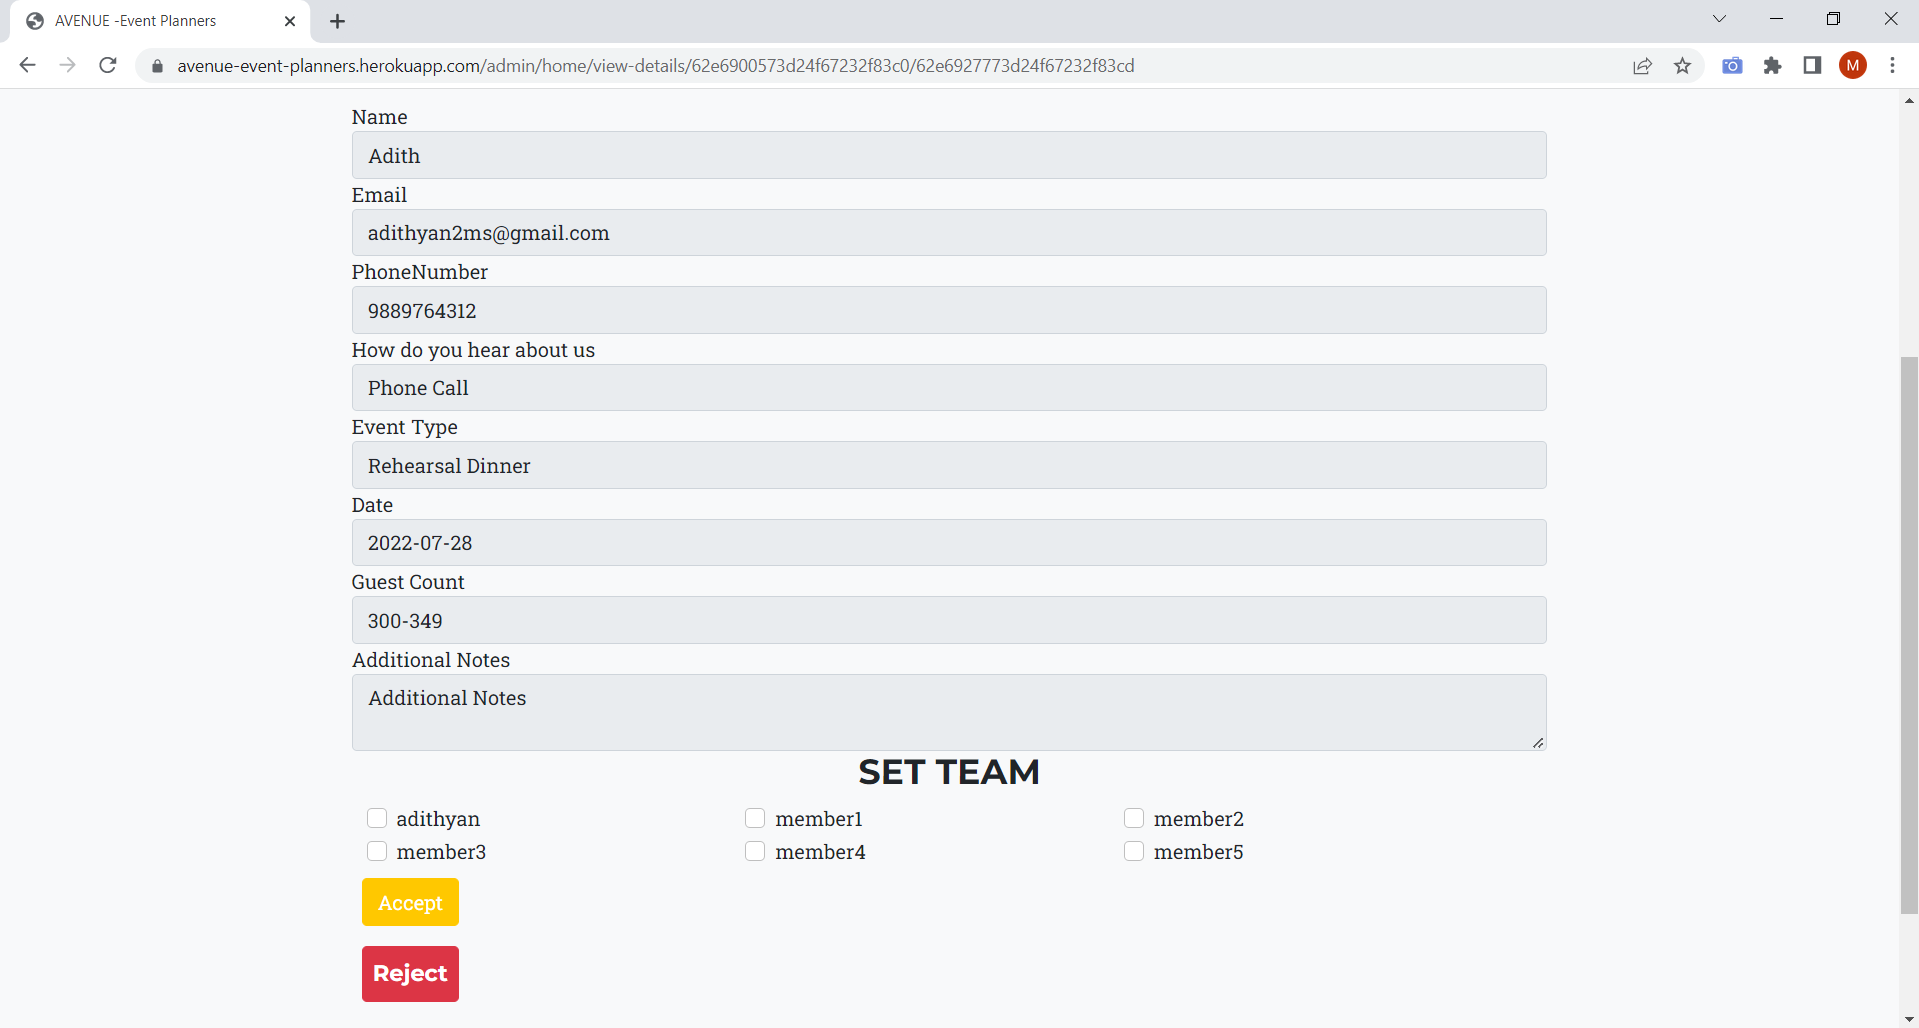
\includegraphics[scale=0.35]{adminview.png}
	\caption{Admin handling event request}
	\label{Admin handling event request}
\end{figure}
\subsection{Scheduled Events}
Events accepted by the admin are shown here containing the event details and the team members.
\begin{figure}[H]
	\centering
	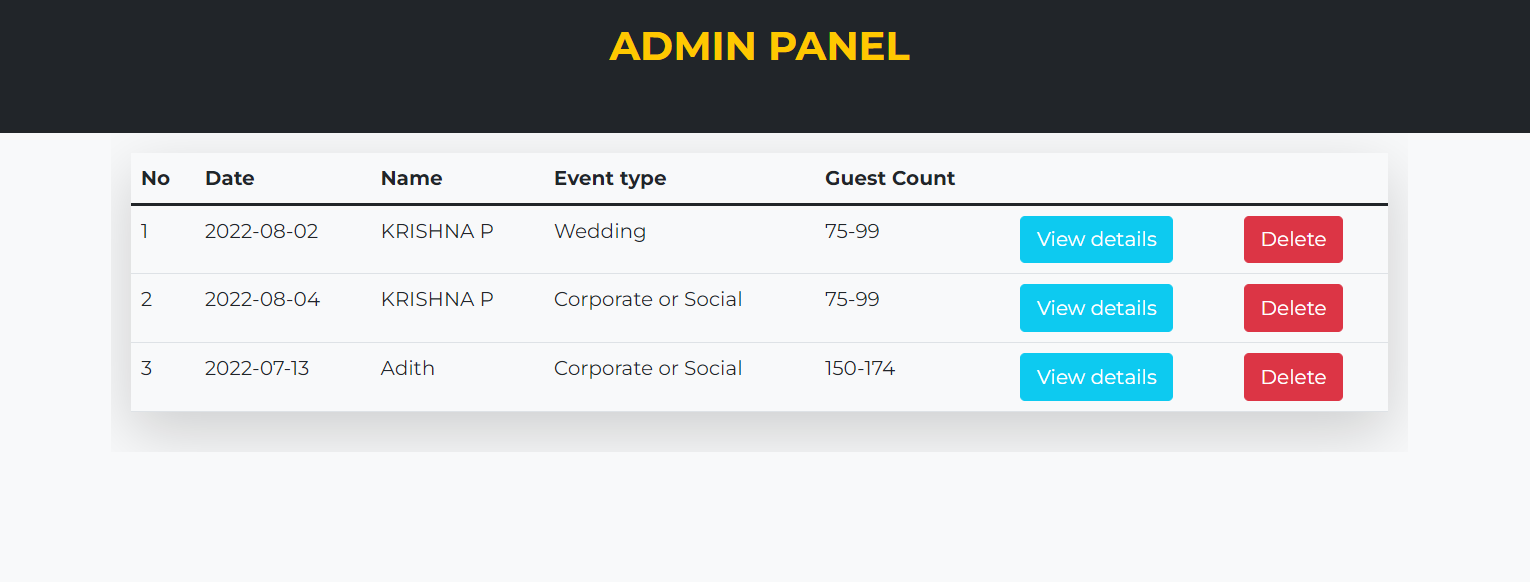
\includegraphics[scale=0.35]{scheduledevents.png}
	\caption{Scheduled Event Page}
	\label{Scheduled Event Page}
\end{figure}
\subsection{Adding Event Planners}
Admin adds new event planners details. After adding the details the login creditionals for the member's account are mailed to the planner's mailid.
\begin{figure}[H]
	\centering
	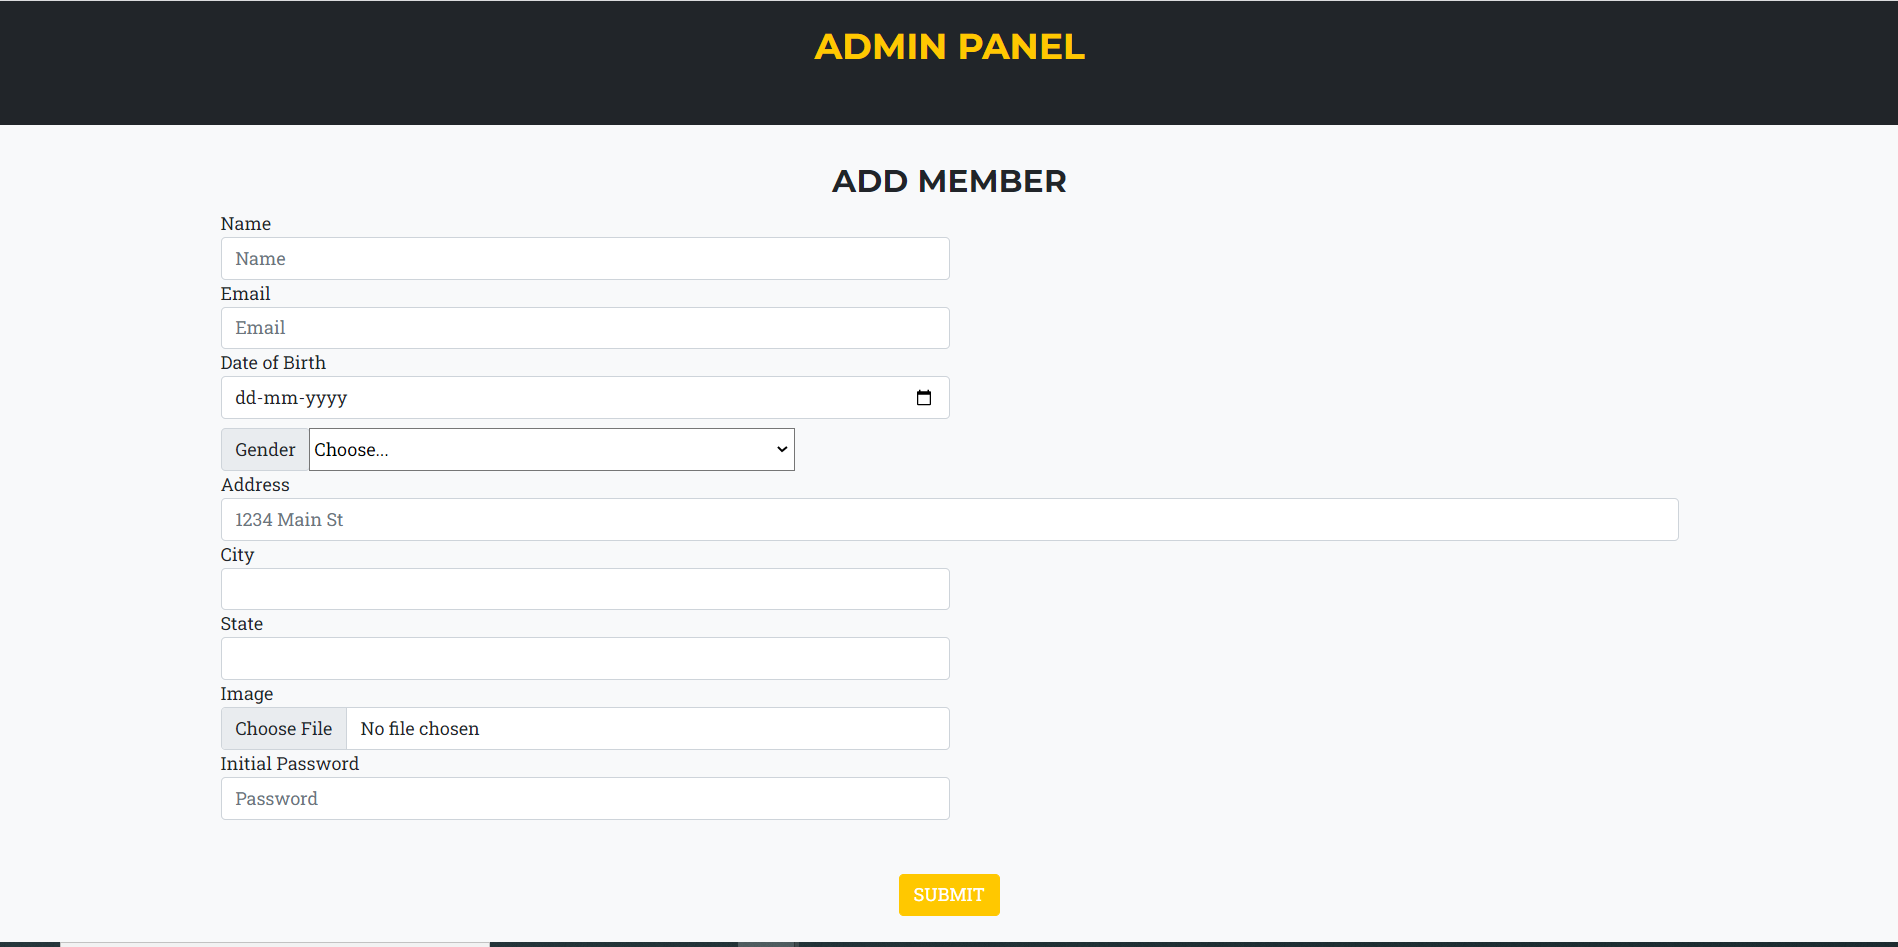
\includegraphics[scale=0.35]{addmember.png}
	\caption{Adding Members Page}
	\label{Adding Members Page}
\end{figure}
\subsection{Adding Portfolio Images}
Portfolio Images for the website added by the admins so that new event images can be updated occasionally.
\begin{figure}[H]
	\centering
	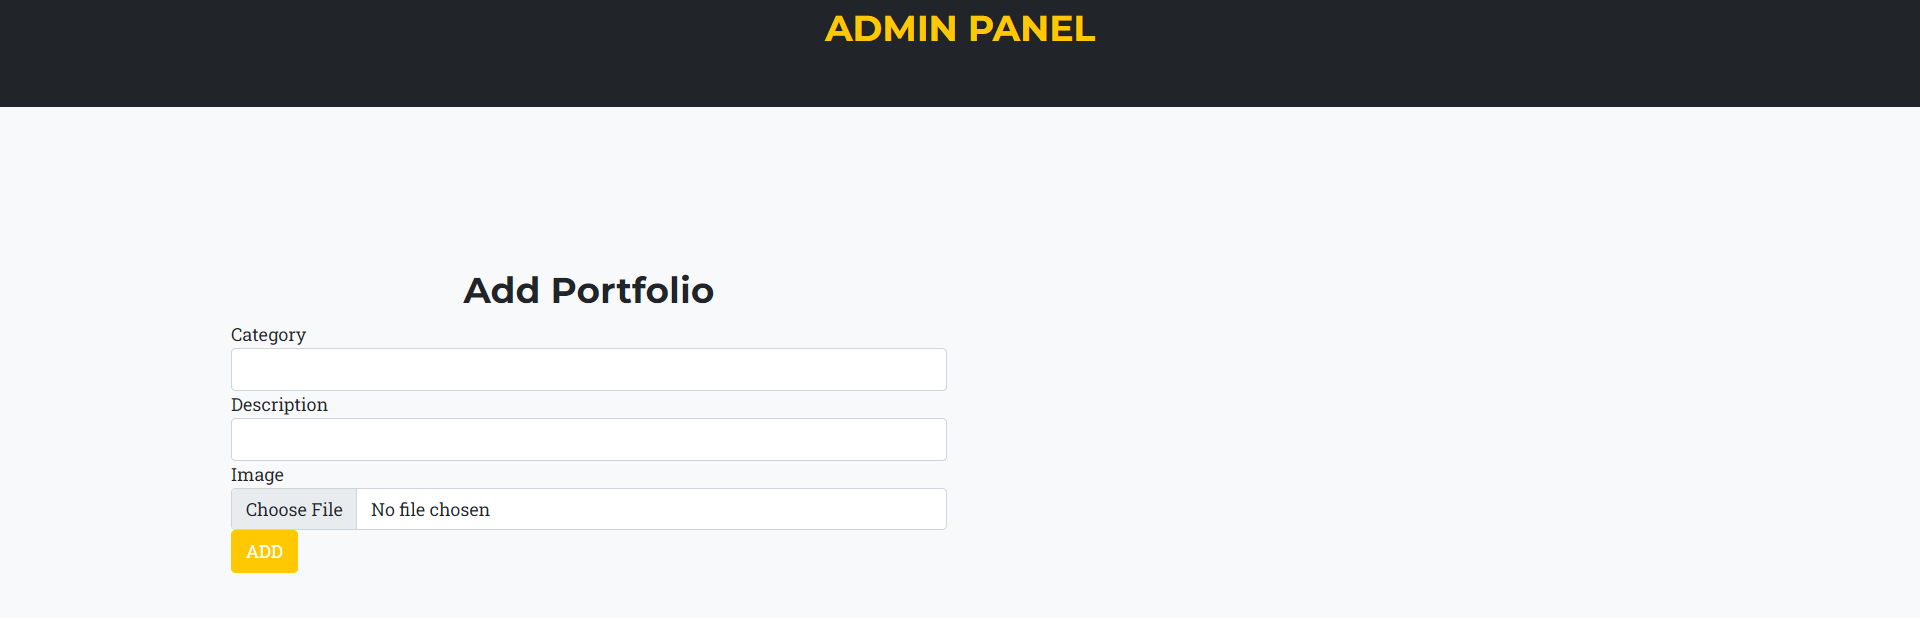
\includegraphics[scale=0.35]{addportfolio.png}
	\caption{Add Portfolio images Page}
	\label{Add Portfolio images Page}
\end{figure}
\subsection{Chat Page}
Once the event has been scheduled the client can chat with the event planners using the chat interface.
\begin{figure}[H]
	\centering
	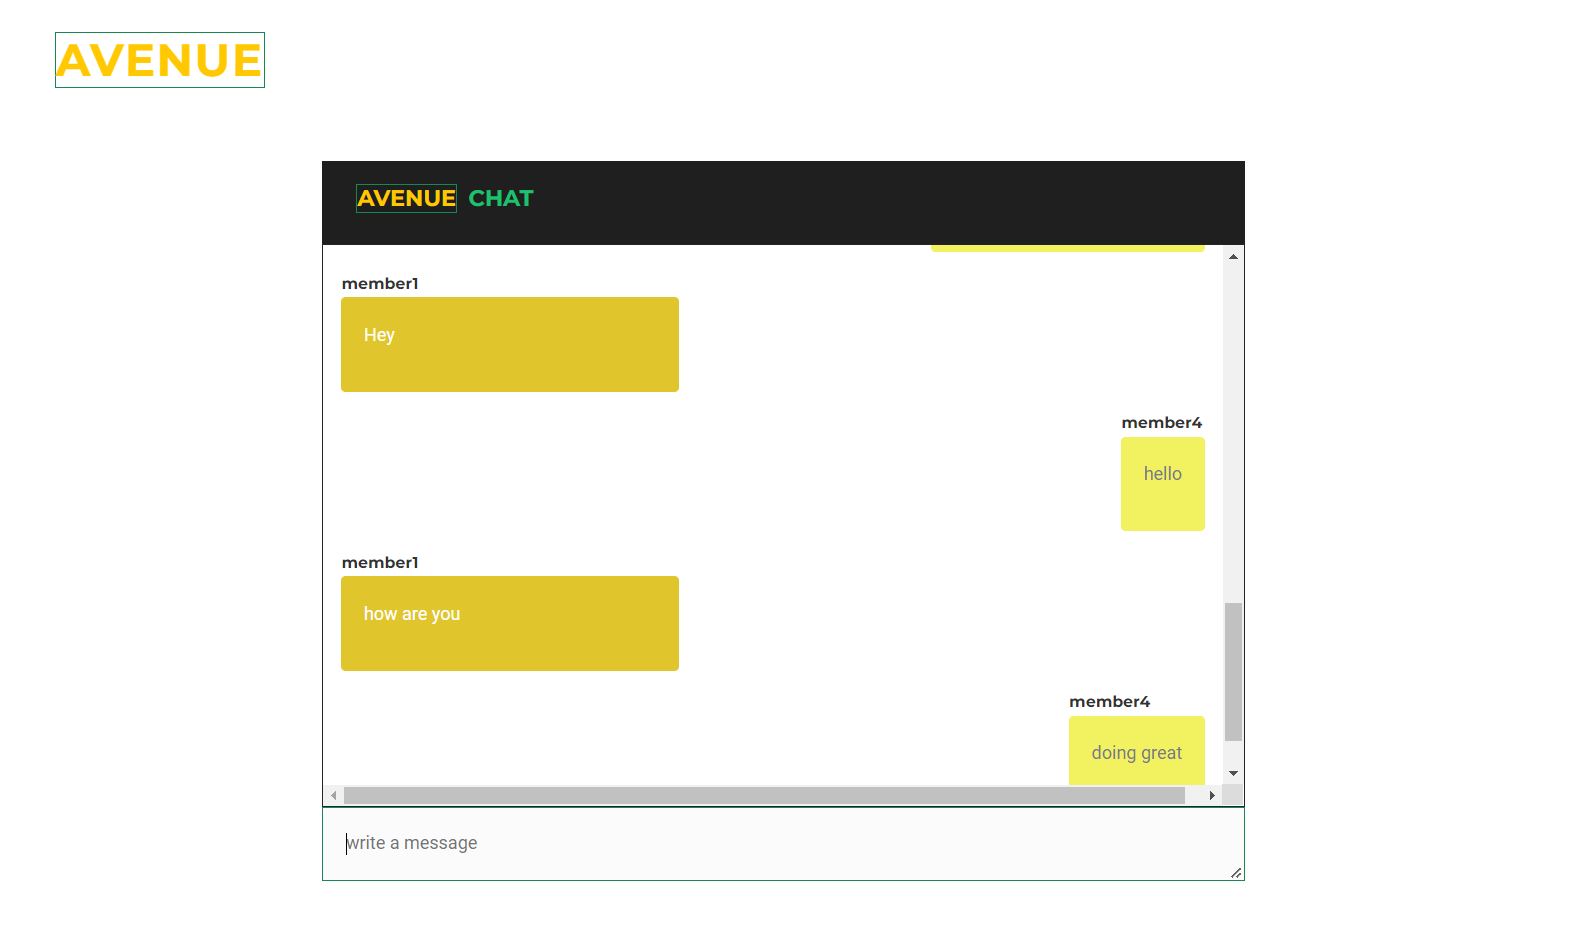
\includegraphics[scale=0.4]{chatpage.png}
	\caption{Chat Page}
	\label{Chat Page}
\end{figure}

\section{Discussion of Results   }
The main objective of the research project was to design and develop an online event management system. The project aim was automating the processes of booking and handling the events at Avenue Event Managem
through the Design and Development of an online event management system.
\newline
A number of steps are summarized in terms of the four specific objectives. The achievement of these specific objectives is explained
below; 
 \newline
The first specific objective was to review the current event managements system. This
was done in chapter two where a number of literatures relating to the research problem
were reviewed which helped in identifying the gaps in the related work that was already
done by other researchers \newline
The requirements of the proposed system i.e. user and system requirements were
collected and analyzed using different methodologies as discussed in chapter three. The proposed system requirements and the system designs are also explained in the same chapter.
\newline
The third specific objective was to develop the online Event Management System. The
System was developed basing on the designs presented in chapter 3, Software
tools like NodeJS, MongoDB, HTML ,CSS and JavaScript were used in the development
process. \newline
All the activities mentioned above were done with the main aim of achieving what was
proposed.













\chapter{CONCLUSION}
\thispagestyle{empty}
\par Phishing detection is now an area of great interest among the researchers due to its significance in protecting privacy and providing security. There are many methods that perform phishing detection by classification of websites using trained machine learning models. URL based analysis increases the speed of detection. Furthermore, by applying feature selection algorithms and dimensionality reduction techniques, we can reduce the number of features and remove irrelevant data. There are many machine learning algorithms that perform classification with good performance measures and we choose the most accurate among them. 

%\newpage
\addcontentsline{toc}{chapter}{REFERENCES}
\begin{thebibliography}{99}
	\bibitem{1} "PhishHaven—An Efficient Real-Time AI Phishing URLs Detection System" ( Maria Sameen, Kyunghyun Han, Seong Oun Hwang [2020])
	
	\bibitem{2}
	"Sufficiency of Ensemble Machine Learning Methods for Phishing Websites Detection"
	(Yi Wei, Yuji Sekiya. [2021])
	
	\bibitem{3}
	"Eth-PSD: A Machine Learning-Based Phishing Scam Detection Approach in Ethereum" (Arkan Hammoodi Hasan Kabla, Mohammed Anbar, Selvakumar Manickam, Shankar Karupayah
. [2021])
	
	\bibitem{4}
	"OFS-NN: An Effective Phishing Websites Detection Model Based on Optimal Feature Selection and Neural Network" (Erzhou Zhu, Yuyang Chen, Chengcheng Ye, Xuejun Li, Feng Liu. [2019])
	
	\bibitem{5}
	"Comparison of Classification Algorithms for Detection of Phishing Websites" (Paulius Vaitkevicius. [2020])
	
	\bibitem{6}
	"Phishing Detection using Random Forest, SVM and Neural Network with Backpropagation" (Sindhu, Sunil Parameshwar Patil, Arya Sreevalsan,  Faiz Rahman	[2020])
	
	\bibitem{7}
	"Intelligent rule-based phishing websites classification" (Rami M. Mohammad, Fadi Thabtah, Lee McLusky. [2014])
	
	\bibitem{8}
	"Phishing sites detection based on Url Correlation" (Ying Xue, Yang Li,Yuangang Yao, Xianghui Zhao, Jianyi Liu,Ru Zhang. [2016])
	\bibitem{9}
	"Characteristics of Understanding URLs and Domain Names Features: The Detection of Phishing Websites With Machine Learning Methods" (Ilker Kara, Murathan Ok, Ahmet Ozaday
. [2022])
	\bibitem{10}
	"Detecting phishing websites using machine learning technique" (Ashit Kumar Dutta, Zhihan Lv. [2018])
	\bibitem{11}
	"Web Phishing Detection Using Machine Learning " (N Kumaran, Purandhar Sri Sai, Lokesh Manikanta. [2022])
	\bibitem{12}
	"Detection of Phishing Websites using Machine Learning" (Atharva Deshpande, Omkar Pedamkar, Nachiket Chaudhary . [2021])
	\bibitem{13}
	A New Method for Detection of Phishing Websites: URL Detection" (Shraddha Parekh,
Dhwanil Parikh ,
Srushti Kotak , Prof. Smita Sankhe. [2018])
	\bibitem{8}
	"Detection of URL based Phishing attacks Using Machine Learning" (Ms. Sophiya Shikalgar , Dr. S. D. Sawarkar , Mrs. Swati Narwane. [2018])
	\bibitem{8}
	"Large-Scale Automatic Classification of Phishing Pages 
" (Collin Whittaker, Brian Ryner, Maria Nasif. [2010])





\end{thebibliography}





%\cite{1,2,3,4,5,6,7,8,9,10,11,12,13,14,15,16,17,18,19,20,21,22,23,24}
%\bibliography{r.bib}
%\bibliographystyle{IEEEtran}
\end{document}
